\documentclass{article}[12pt]
%----------------Package-Only----------
\usepackage{eForceStyle}
% --------------Names-------------
\def\CarNumber{E67}% Car number
\def\UniversityName{CTU Prague}% University Name
\def\Event{2017 Formula Student East}% Event
%--------acronyms
% nezapomen pres nasttroje-prikazy-make glossaries

\makeglossaries

\newacronym{air}{AIR}{accumulator isolation relay}
%\newacronym{airs}{AIRs}{meaning both accumulator isolation relay-s} %instead, use \glspl{air}
\newacronym{ams}{AMS}{accupack management system}
\newacronym{acp}{ACP}{accupack}
\newacronym{bots}{BOTS}{break over travel switch}
\newacronym{bspd}{BSPD}{break system plausability device}
\newacronym{mc}{MC}{motor controller (dual)}
\newacronym{mcf}{MCF}{motor controller - front}
\newacronym{mcr}{MCR}{motor controller - rear}
\newacronym{hv}{HV}{high voltage}
\newacronym{lv}{LV}{low voltage}
\newacronym{imd}{IMD}{isoaltion measuring device}
\newacronym{sdb}{SDB}{shut down button}
\newacronym{sdc}{SDC}{shut down circuit}
%\newacronym{ts}{TS}{traction system - (everything HV that influence motor torque and speed)}
\newacronym{ts}{TS}{traction system}
\newacronym{tsms}{TSMS}{traction system master switch}
\newacronym{vdcu}{VDCU}{vehicle dynamics control unit}
\newacronym{fail}{FAIL}{front Axels InterLock}
\newacronym{ecu}{ECU}{electronic control unit}
\newacronym{ecup}{ECU-P}{electronic control unit - pedals}
\newacronym{ecub}{ECU-B}{electronic control unit - back}
\newacronym{ecus}{ECU-S}{electronic control unit - steering}
\newacronym{ecuf}{ECU-F}{electronic control unit - front}
\newacronym{ecua}{ECU-A}{electronic control unit - accupack}
\newacronym{adc}{ADC}{analog to digital converter}
\newacronym{mcu}{MCU}{microcontroller unit}
\newacronym{can}{CAN}{controller area network}
\newacronym{bms}{BMS}{battery management system}
\newacronym{ntc}{NTC}{negative temperature coeffitient}
\newacronym{pcb}{PCB}{printed circuit board}
\newacronym{glvs}{GLV}{grounded low voltage system}
\newacronym{hw}{HW}{hardware}
\newacronym{fw}{FW}{firmware}
\newacronym{pmsm}{PMSM}{permanent magnet synchornous motor}

%\makeglossaries
\glsaddall
\begin{document}

%--------titlepage-------
	\begin{titlepage}
			\centering	
\includegraphics[width=\textwidth, trim={0cm 6cm 0cm 20cm}, clip]{./img/title-logo.pdf}
\vspace{.5cm}
{\scshape\huge Electrical Safety Form FSAE-E 2018 \par}
\vspace{.5cm}
%\includegraphics[width=\textwidth, trim={0cm 150cm 150cm 0cm}, clip]{./img/title-cover.pdf}	
%\vspace{.5cm}
%\vspace{1cm}
{\scshape\Large Czech Technical University in Prague\par}
%\vspace{1cm}
\vspace{.5cm}
{\LARGE eForce FEE Prague Formula\par}
%\vspace{1cm}
\vspace{.9cm}
{\LARGE E67\par}
%\vspace{1cm}
\vspace{.6cm}

\begin{table}[H]
	\centering
	%\flushright
	\begin{tabular}{rl}
		ESF responsible: &  \href{mailto:ondrej.sereda@eforce.cvut.cz}{Ondrej Sereda}  \\
		Team Captain: & Jan Kosina   \\
	\end{tabular}%
	\label{tab:title}%
\end{table}%

%{\large\itshape ESF responsible: Lukas Hostacny, email: lukas.hostacny@eforce.cvut.cz\\
%	Cc: Jan Kosina, email: jan.kosina@eforce.cvut.cz\par}


\vfill
	\end{titlepage}
%--------table of contens--------------------------------------
\pagenumbering{Roman}
%\sectionnumbering{Roman}
\setcounter{page}{1}

\tableofcontents
\addcontentsline{toc}{section}{\contentsname}  
\newpage
 % List of Figures
	%\pagenumbering{roman} This is just Stupid
\listoffigures
\addcontentsline{toc}{section}{I\quad\listfigurename} 
\newpage
% List of Tables
\listoftables
\addcontentsline{toc}{section}{II \thinspace\thinspace \listtablename} 
\newpage
% List of Acronyms
\printglossary[type=\acronymtype,title=List of Acronyms]\begin{flushleft}
	
\end{flushleft}
\addcontentsline{toc}{section}{III List of Acronyms} 
\newpage

%\cleardoubleoddpage
\pagenumbering{arabic}
%\sectionnumbering{arabic}
%\setcounter{page}{1}
%-------ESF---------------------------------------------------
\section{System Overview}

Electrical systems of the car are divided into small blocks. The concept is to have all the systems distributed by 2 \gls{can} buses (1st “CAN\_Powertrain” for systems crucial data to proper function, 2nd “CAN\_Aux” for all the other systems) and, if possible, all the signals transferred just by \gls{can} bus. Baud rate is 500kbps and \gls{can} is terminated in \gls{ecup} in front of car and in \gls{mcf} by 120$\Omega$ resistor. There are in total 5 main control units – of course all the units are fully self-made (\gls{hw} and \gls{fw}).

\begin{itemize}
\item	\Glsdesc{ecup}
This device measures brake pedal and acceleration pedal positions, implements safety algorithms regarding to rules about torque encoder check and outputs these values to the CAN bus as driver’s foot requests. It also monitors Shutdown Circuit – point BOTS. 

\item	\Glsdesc{vdcu}
This device reads driver’s foot requests, actual every wheel speed provided by ECUM and implements Traction Control Algorithms. The result is sent over private \gls{can} bus to the \gls{mcf} and \gls{mcr}. 

\item	\Glsdesc{mc}
2 units in total – \gls{mcf} and \gls{mcr}. These units drives 4 motors in total, so every unit drives 2 motors. It provides speed of every wheel by actual RPM, temperatures and so on. Field Oriented Control is implemented with Resolvers as a position feedbacks.

\item	\Glsdesc{ecuf} (+ Dashboard)
Interaction with driver in cooperation with \gls{ecus} (LCD inside) by informing, warning and error LEDs, switches, rotary switches, push buttons. This is like a driver’s \gls{can} bus console. 

\item	\Glsdesc{ecub}
Providing low voltage power distribution to all the control units and periphery (Li-Ion \gls{lv} battery with \gls{bms} inside). This unit implements all the safety and control algorithms regarding to Shutdown Circuit rules. The main function is to latch \gls{sdc} and evaluation of \gls{sdc} interruption point. 

\item	\Glsdesc{ecua}
DC-DC converter, \gls{bms}, Pre-charge and \gls{air} controlling is implemented. This unit also communicate with Charging Station.

There are other control and measuring systems not listed above, but these systems are most important for safety and control.

\end{itemize}

There are other control and measuring systems not listed above, but systems listed are most important for safety and control.

%\item Short description of the system’s concept 
%\item Rough Schematic (blocks) showing all parts affected with the electrical systems and function of the tractive-system
%\item No detailed wiring
%\item Additionally, fill out the following table, replacing the values with your specifications:

\begin{table}[H]
	\centering
	\caption{General parameters}
	\begin{tabularx}{\textwidth}{|X|X|}
		\hline
		Maximum Tractive-system voltage: & 400 $V_{DC}$  \\[\TableSize]
		\hline Nominal Tractive-system voltage: & 345.6 $V_{DC}$\\[\TableSize]
		\hline
		Control-system voltage: & 24 $V_{DC}$ \\[\TableSize]
		\hline
		Accumulator configuration: & 96s9p \\[\TableSize]
		\hline
		Total Accumulator capacity: & 7.78 kWh\\[\TableSize]
		\hline
		Nominal HV Accumulator current: & 270 A \\[\TableSize]
		\hline
		Maximum HV Accumulator current: & 315 A \\[\TableSize]
		\hline
		HV accumulator cell type: & Lithium-Ion  \\[\TableSize]
		\hline
		LV Accumulator cell type: & Lithium-In \\[\TableSize]
		\hline
		Motor type: & \gls{pmsm} with resolvers \\[\TableSize]
		\hline
		Number of motors: &  4, one per wheel \\[\TableSize]
		\hline
		Maximum combined motor power in kW & 109 \\[\TableSize]
		\hline
	\end{tabularx}%
	\label{tab:system-general}%
\end{table}%


\section{Electrical Systems}
% chybi obrazky a schema sdc a pozice v aute
\subsection{Shutdown Circuit}\label{subsec:SDC}
% This is copied from 2017 ESF and it is example of LaTex
% -------------------------------------------------------
% Ondřej Šereda 8.2.2018

\subsubsection{Description/concept}
\iffalse
Describe your concept of the shutdown circuit, the master switches, shut down buttons, brake over travel switch, etc.
Additionally, fill out the following table replacing the values with your specification and append additional switches from your setup:
\fi

Shutdown circuit (SDC) starts in ECUP unit, then goes through all SDC elements in the car and ends in ECUA, which is placed inside the Accumulator Pack. In ECUP SDC starts from LV power +24V and ends in ACP by powering AIR coils switching circuit (See \ref{fig:SDC-scheme}). The SDC consists of 2 master switches, 3 shut-down buttons(SDB), the brake-over-travel-switch(BOTS), the insulation monitoring device (IMD), the inertia switch, the brake system plausibility device(BSPD), interlocks in Motor Controllers and Accumulator Pack and the accumulator management system (AMS). All of these crucial parts do not act through any power stage, but carry directly the AIR current.

\begin{figure}[H]
	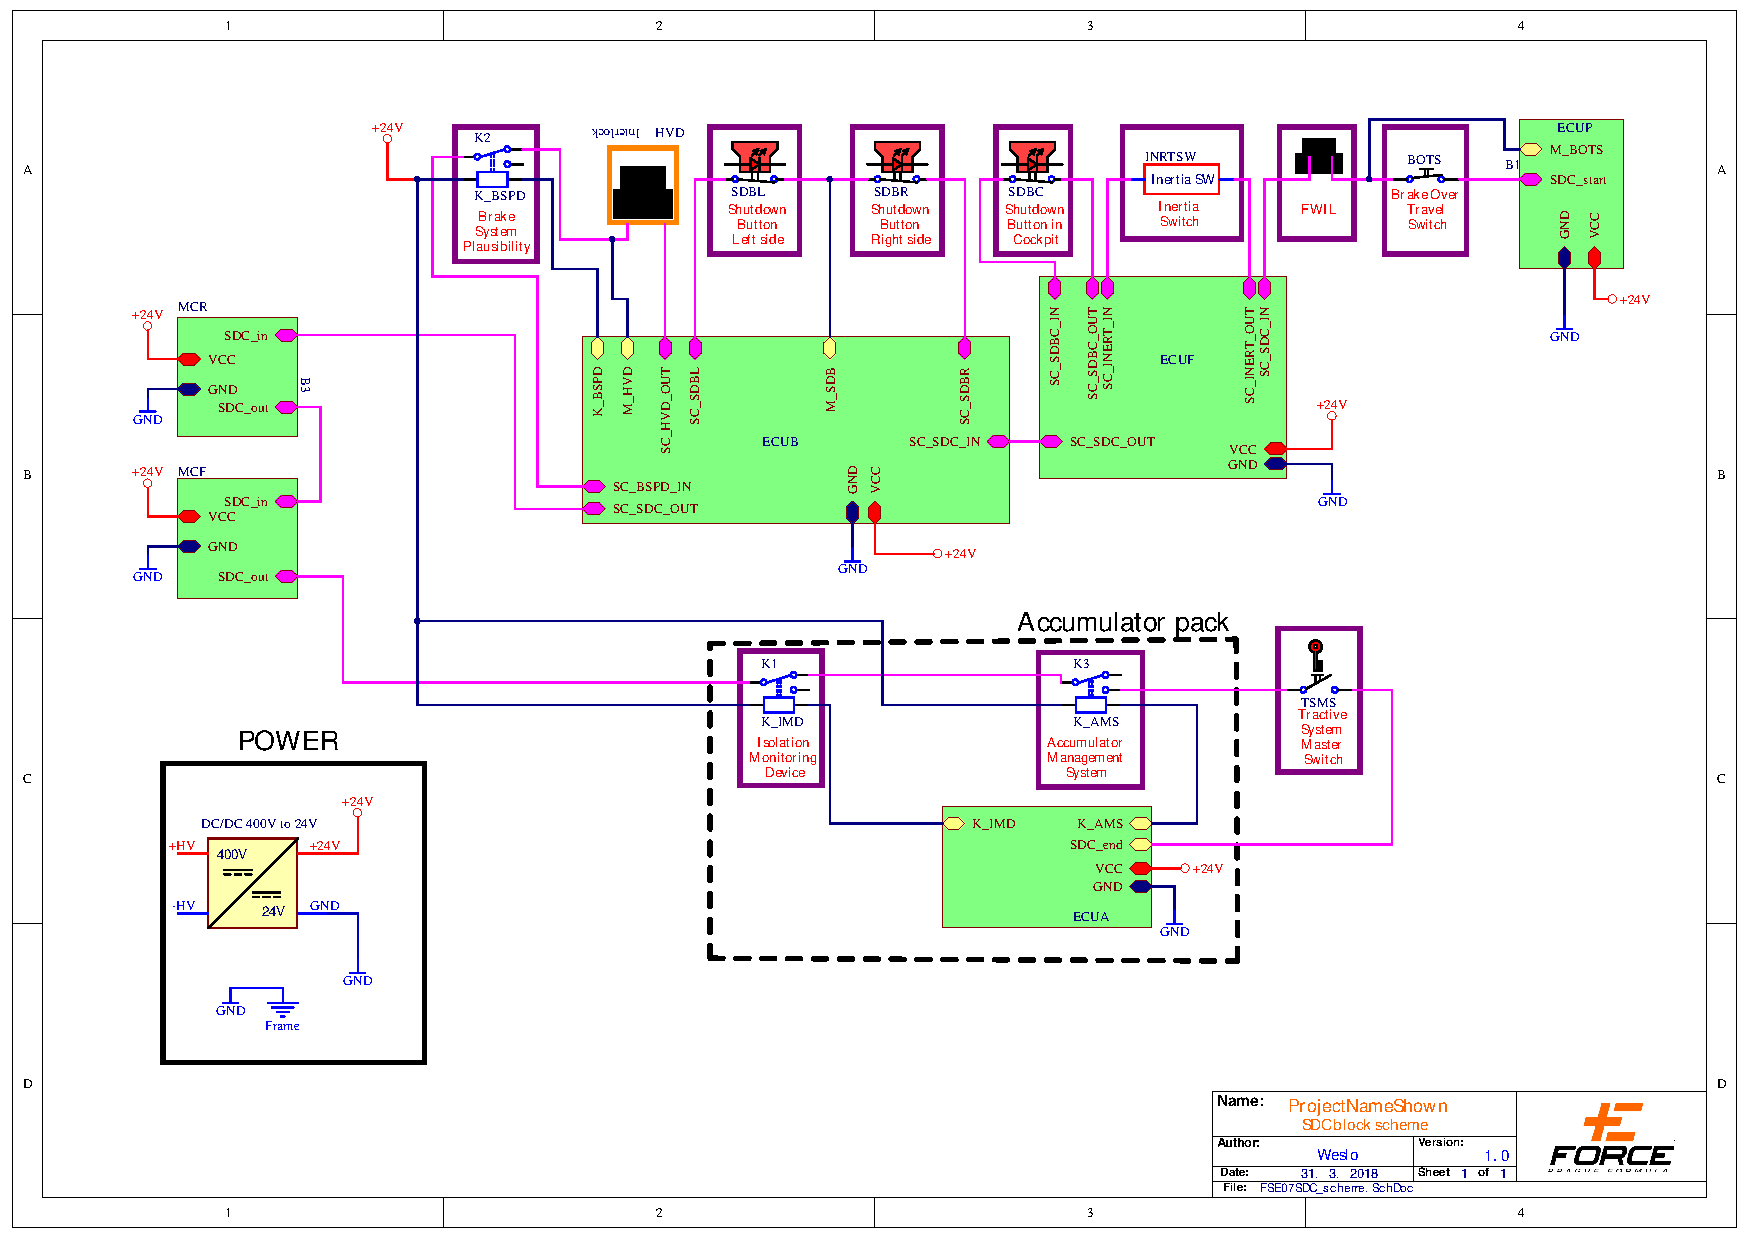
\includegraphics[width=\textwidth, trim={2cm 3cm 2cm 2cm},clip]{./img/SDC-scheme.pdf}
	\caption{SDC scheme.}
	\label{fig:SDC-scheme}
\end{figure}

\begin{table}[H]
	\caption{List of switches in the shutdown circuit}
	\centering
	\begin{tabularx}{\textwidth}{|X|l|}
		\hline Part  & Function \\[\TableSize]
		\hline Main Switch (for control and tractive-system; CSMS, TSMS) & Normally open \\[\TableSize]
		\hline Brake over travel switch (BOTS) & Normally closed \\[\TableSize]
		\hline Shutdown buttons (SDB) & Normally closed \\[\TableSize]
		\hline Insulation Monitoring Device (IMD) & Normally open \\[\TableSize]
		\hline Battery Management System (BMS) & Normally open \\[\TableSize]
		\hline Inertia Switch & Normally closed \\[\TableSize]
		\hline Interlocks & Closed when circuits are connected \\[\TableSize]
		\hline Brake System Plausibility Device & Normally Open \\[\TableSize]
		\hline
	\end{tabularx}%
	\label{tab:SDCswitch}%
\end{table}%


\paragraph{Monitoring SDC}
Every part of \gls{sdc} is monitored by specific \gls{ecu} in order to identify disconnected element. \gls{bots} is measured by \gls{ecup}, SDB-center  and Inertia switch are measured by \gls{ecuf} , interlocks in \glspl{mc} (\gls{fwil}) are measured by \glspl{mc}, Interlock in Accumulator Pack is measured by \gls{ecua}  and finally SDB-right, SDB-left and \gls{tsms} are measured by \gls{ecub}. Every piece of information regarding the state of closure \gls{sdc} are running between ECU´s by \gls{can}. 

We designed \gls{sdc} to be ‘single wire’ alike and distanced it from the system as much as it was possible. In order to remain \gls{sdc} as a stand-alone wire we used optocouplers for main points of \gls{sdc}. Optocouplers are connected in such a way, that they become active only in case of nonzero voltage occurance at a certain point of \gls{sdc}.

\Gls{ecub} is last part of \gls{sdc} before \gls{tsms}. If a state of error on \gls{sdc} is detected \gls{ecub} latches the off-state of \gls{sdc} to stay off. If the occurred error is non-critical, it allows pilot to re-enter the TSON state. If monitored error is critical (such as \gls{imd} etc.), it notes the error to the memory-storage and does not allow \gls{sdc} to become active until appropriate steps are taken.

\paragraph{Master Switch}
We use SCI A23-5 battery cut-out switches with continuous current rating 100A, shown on \ref{fig:SDC-TSMS}.
\begin{figure}[H]
	\centering
	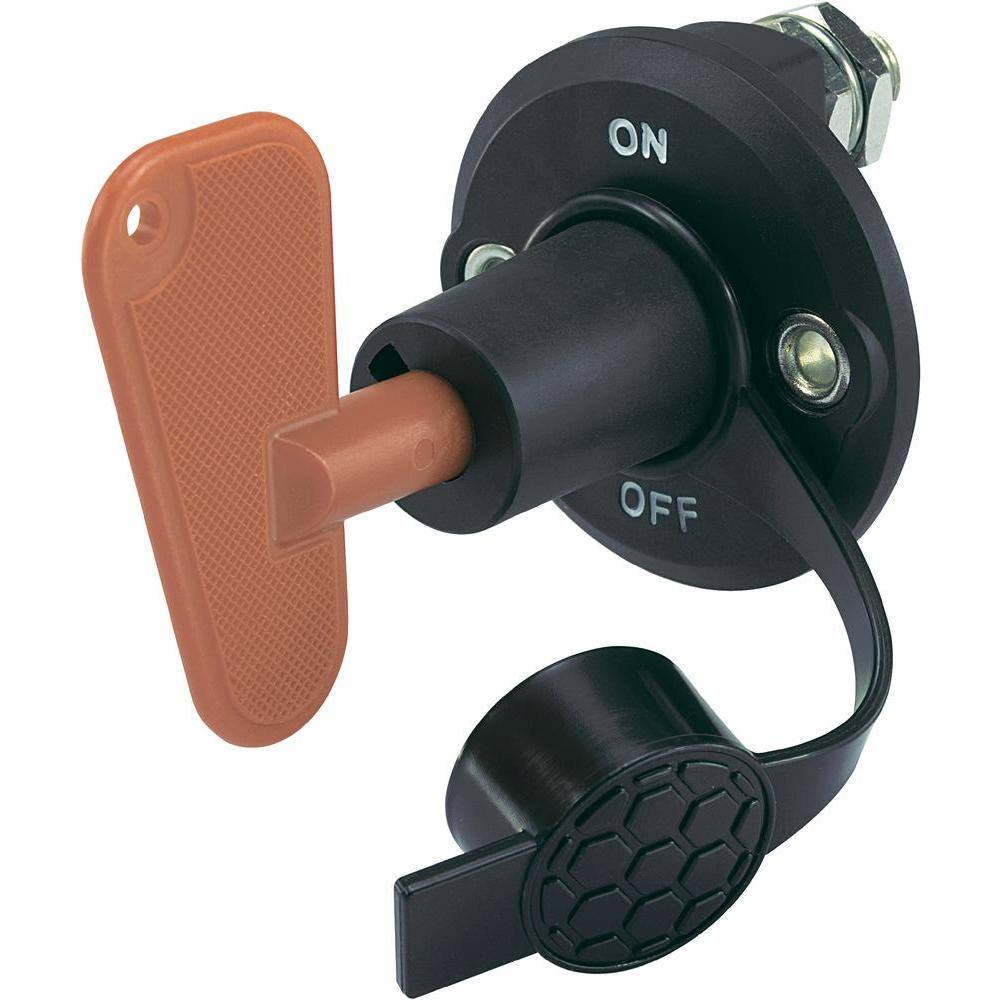
\includegraphics[width=.5\textwidth]{./img/SDC-TSMS.jpg}
	\caption{TSMS.}
	\label{fig:SDC-TSMS}
\end{figure}

\paragraph{Shutdown Switch}
We use OMRON A165E shutdown buttons, which have 3A current rating at 30VDC.

On the cockpit it is OMRON A165E-LS, shown on \ref{fig:SDC-A165E-LS}.
\begin{figure}[H]
	\centering
	\includegraphics[width=.5\textwidth]{./img/SDC-A165E-LS.pdf}
	\caption{Cockpit SDB.}
	\label{fig:SDC-A165E-LS}
\end{figure}

On the left and on the right sides there are OMRON A165E-LM buttons, shown on \ref{fig:SDC-A165E-LM}.
\begin{figure}[H]
	\centering
	\includegraphics[width=.5\textwidth]{./img/SDC-A165E-LM.pdf}
	\caption{SDB left and right.}
	\label{fig:SDC-A165E-LM}
\end{figure}

\paragraph{Brake Over Travel Switch}
It is type A165E-M, current raging 3A, shown on \ref{fig:SDC-A165E-M}
\begin{figure}[H]
	\centering
	\includegraphics[width=.5\textwidth]{./img/SDC-A165E-M.pdf}
	\caption{Brake over travel switch.}
	\label{fig:SDC-A165E-M}
\end{figure}


\subsubsection{Wiring / additional circuitry}
\iffalse
Describe wiring and additional circuitry, show extra schematics for example if additional transistors etc. are used, also describe the function of additional circuitry and make good use of figures.
Additionally, fill out and add information to the following table:
\fi

If connector is used to connect \gls{sdc} between control units, disconnecting any of them results in opening \gls{sdc} and therefore opening \glspl{air} as well. In other words the \gls{sdc} directly carries the current driving the accumulator isolation relays(\glspl{air}). All circuits that are part of the shutdown circuit have been designed in a way, that, when in disconnected state, they remove the current controlling the \glspl{air}.

The cross-section of Shutdown System wire is AWG22. Block wiring scheme shown on \ref{fig:SDC-schematic}.\\

\begin{figure}[H]
	\centering
	\includegraphics[width=\textwidth,trim={4cm 8cm 5cm 3cm}, clip]{./img/SDC-monitoring.pdf}
	\caption{Example of used \gls{sdc} monitoring method with optocouplers.}
	\label{fig:SDC-schematic}
\end{figure}

As shown, 4k7 resistors are used to limit current through optocoupler. With 24V supply that makes 15,2mA per optocoupler. We used 8 optocouplers => 12*15, 2= 182,4mA.
% Table generated by Excel2LaTeX from sheet 'List1'
\begin{table}[H]
	\centering
	\caption{Wiring – Shutdown circuit}
	\begin{tabularx}{\textwidth}{|X|X|}
		\hline
		Total Number of \glspl{air}: & 2 \\[\TableSize]
		\hline
		Current per \gls{air}: & 70 mA \\[\TableSize]
		\hline
		Additional parts consumption within the shutdown circuit: & 182.4 mA \\[\TableSize]
		\hline
		Total current: & 322.4 mA \\[\TableSize]
		\hline
		Cross sectional area of the wiring used: & 0.322 mm$^2$ (AWG22) \\[\TableSize]
		\hline
	\end{tabularx}%
	\label{tab:SDC-Wiring}%
\end{table}%


\subsubsection{Position in car}
\iffalse Provide CAD-renderings showing the relevant parts. Mark the parts in the renderings, if necessary. \fi
\begin{figure}[H]
	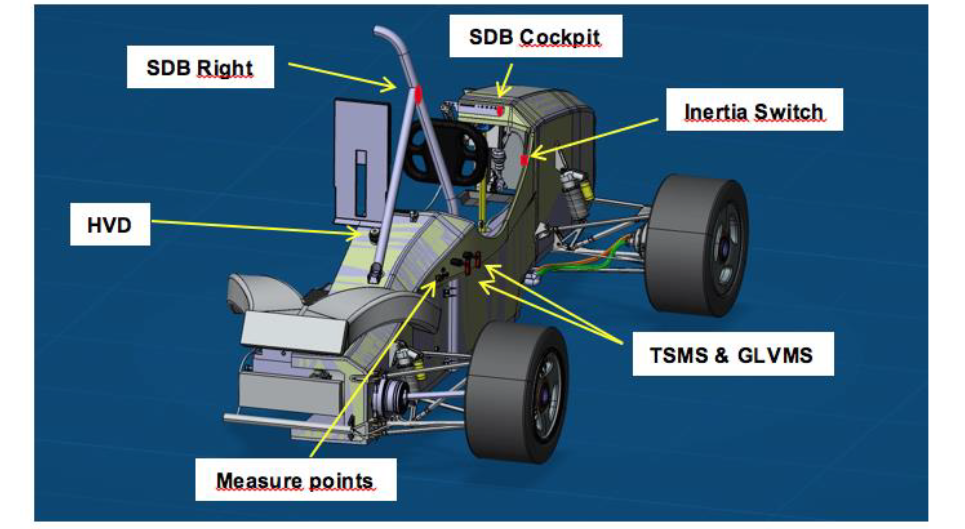
\includegraphics[width=\textwidth]{./img/SDC-positionInCar.png}
	\caption{Inertia switch, SDB Left, Right and Cockpit, \gls{tsms}, \gls{glvms}, HVD, Measure points.}
	\label{fig:SDC-positionInCar}
\end{figure}


\subsection{IMD}
% chybi tady reference na datasheet
\subsubsection{Description (type, operation parameters)}
\iffalse Describe the IMD used and use a table for the common operation parameters, like supply voltage, set point, etc. Also, describe how the IMD indicator light is wired, etc.
Additionally, fill out the following table replacing the values with your specification:\fi

We use A-ISOMETER® IR155-3203 Insulation monitoring device (IMD) for unearthed DC drive systems. Our maximum tractive voltage is 403.2 VDC. The rules require minimal insulation value between TS and GLVS 500 Ohm/V. Minimal resistance value for our car is 408*500 = 204 000 Ohm. This was set as request for manufacturer, and device was programmed in factory.
\begin{table}[H]
	\centering
	\caption{Parameters of the IMD}
	\begin{tabu}{|X|l|}
	 \hline	Supply voltage range: & 10..36VDC \\
	 \hline	Supply voltage & 24VDC \\
	 \hline	Environmental temperature range: & -40..105°C \\
	 \hline	Selftest interval: & Always at startup, then every 5 minutes \\
	 \hline	High voltage range: & DC 0..1000V \\
	 \hline	Set response value: & 204kΩ (500Ω/Volt) \\
	 \hline	Max. operation current: & 150mA \\
	 \hline	Approximate time to shut down at 50\% of the response value: & 20s \\
	  \hline
	\end{tabu}%
	\label{tab:IMD}%
\end{table}%

\subsubsection{Wiring/cables/connectors/}
 Describe wiring, show schematics, describe connectors and cables used and show useful data regarding the wiring including wire gauge/temp/voltage rating and fuses protecting the wiring. 

Relay of Insulation Monitoring Device is electrically placed between MCF and relay for AMS measurement. Wiring is done using Raychem Spec44 wire, AWG 22, rated to 600V. Wiring is shown on \ref{fig:SDC-scheme}. IMD opens relay in case of fault. IMD have output for relay, so there is not necessary adding zero diode on output. HV input to IMD is connected in according to datasheet.

\subsubsection{Position in car}
% Provide CAD-renderings showing the relevant parts. Mark the parts in the rendering, if necessary

\begin{figure}[H]
	\centering
	\includegraphics[width=\textwidth,trim={0cm 0cm 0cm 0cm},clip]{./img/IMD-position.jpg}
	\caption{IMD position.}
	\label{fig:IMD-position}
\end{figure}
\label{sebsec:IMD}

\subsection{Inertia Switch} \label{subsec:InertiaSwitch}
% nefunguje odakzy
\subsubsection{Description (type, operation parameters)}
\iffalse Describe the Inertia Switch used and use a table for the common operation parameters, like supply voltage, temperature, etc.
Additionally, fill out the following table replacing the values with your specification: \fi

Inertia switch opens shutdown circuit in case of acceleration more than 6g. After acting the driver can reset this switch.
\begin{table}[H]
	\centering
	\caption{Parameters of the Inertia Switch}
	\begin{tabularx}{\textwidth}{|X|l|}
	\hline	Inertia Switch type: & Sensata 510FCS01-01 \\[\TableSize]
	\hline	Supply voltage range: & No supply needed \\[\TableSize]
	\hline	Supply voltage: & No supply needed \\[\TableSize]
	\hline	Environmental temperature range: & -30 $^\circ$ 120 $^\circ$C \\[\TableSize]
	\hline	Max. operation current: & 10 A \\[\TableSize]
	\hline	Trigger characteristics: & 6 g for 60 ms / 11 g for 15 ms \\[\TableSize]
	\hline
	\end{tabularx}%
	\label{tab:inertiaSwitch}%
\end{table}%


\subsubsection{Wiring/cables/connectors}
%Describe wiring, show schematics, describe connectors and cables used and show useful data regarding the wiring.

Inertia switch is electrically placed between Shutdown button center on dashboard and the Shutdown input to \gls{ecub}, where is connected right Shutdown button on main hoop. Inertia switch will be connected by FQCT connectors. Wiring of inertia switch is shown on \ref{fig:SDC-scheme}. Wiring of inertia switch is shown on \ref{fig:SDC-scheme}.
\subsubsection{Position in car}
%Provide CAD-renderings showing the relevant parts. Mark the parts in the rendering, if necessary.

Inertia switch is placed on the right side in the cockpit clearly shown in \ref{fig:SDC-positionInCar}.

\subsection{Brake Plausability Device} \label{subsec:BSPD}
% Responsible: Mark G.
% Author: Mark G.

\subsubsection{Description/additional circuitry}
% Describe how your electronic hardware brake plausibility system works (this is in addition to your ECU controlled brake plausibility software), provide tables with main operation parameters, and describe additional circuitry used to check or for an implausibility. Describe how the system reacts if an implausibility or error is detected.

\Gls{bspd} is represented by a \gls{pcb} with an on-board current transducer. It’s function is to monitor
power drawn from \gls{acp} and brake pedal pressure, and open \gls{sdc} in case both signals are above
allowed threshold for more than 0.5 seconds. Also, the event of disconnection of \gls{sdc} is latched,
thus it gets to reset only in case of the main power reset.


\begin{table}[H]
	\centering
	\caption{BSPD data}
	\begin{tabu}{|X|X|}
		\hline
		Brake sensor used: & Piezoresistive Pressure Transmitter PA-21Y / 100bar / 81691.1 \\
		\hline
		Brake sensor physical response value: & Voltage, 4.5V \\
		\hline
		Tractive system power sensor type & Current Transducer LEM HTFS 200-P \\
		\hline
		Tractive system sensor physical response value: & Voltage of 85 mV \\
		\hline
		Tractive System power sensor current threshold (5kW/Nominal \gls{ts} voltage): & 14 A \\
		\hline
		Supply voltages: & 5 V \\
		\hline
		Maximum supply currents: & 22 mA \\
		\hline
		Operating temperature: & -40 $^\circ$C to 105 $^\circ$C \\
		\hline
		Output used to control \glspl{air}: & Open a MOSFET in \gls{sdc} \\
		\hline
	\end{tabu}%
	\label{tab:bspd}%
\end{table}%

Complete datasheet: \ref{app:bspd_lem_datasheet}

\iffalse
\begin{figure}[H]
	\centering
	\includegraphics[width=\textwidth]{./img/bspd-position.jpg}
	\caption{\Gls{bspd} flowchart.}
	\label{fig:BSPD-flowchart}
\end{figure}\fi

\subsubsection{Schematic}
%Describe the wiring, show schematics including the circuit board, show data regarding the cables and connectors used
The \gls{bspd} \gls{pcb} is mounted on a \gls{hv} wire in such manner, that the \gls{hv} wire goes through the
current transducer. Current transducer provides analog voltage output of a value proportional to
actual current (resp. power) drawn from \gls{acp}. This voltage is amplified and is converted to two-state
logic levels voltage with the use of comparators. The value of “High” current signal logic level
is set to be at 5kW of power drawn from \gls{acp} (14A).

Brake state is measured in \gls{ecup}, converted with help of a comparator to two-state logic levels
voltage and is sent directly to \gls{bspd} via wiring.

Both logic signals are connected to NAND inputs. When both inputs are at “High” level, a
capacitor $C_1$ starts to charge through resistance $R_{16}$. When voltage on $C_1$ is higher than 2.5V, a
comparator $U_{1B}$ sends signal to open \gls{sdc}.

\begin{figure}[H]
	\centering
	\includegraphics[width=\textwidth]{./img/bspd-schematic.pdf}
	\caption{\gls{bspd} schematic sheet}
	\label{fig:BSPD-schematic}
\end{figure}

\subsubsection{Connection with shutdown circuit}
The connection to \gls{sdc} is provided by an NPN transistor $Q_2$ and a P-Channel MOSFET $Q_1$, that
are connected to act as a “normally-closed” switch in \gls{sdc} loop. Thus in case of a trip event $Q_1$
stops conducting current between Drain and Source. See \ref{fig:BSPD-schematic}.

This state is latched by a latch-circuit, that consists of two NAND gates.

\iffalse
\begin{figure}[H]
	\centering
	\includegraphics[width=\textwidth]{./img/bspd-position.jpg}
	\caption{\gls{bspd} connection with \gls{sdc}.}
	\label{fig:BSPD-conn}
\end{figure}\fi

\subsubsection{Position in car/mechanical fastening/mechanical connection}
%Provide CAD-renderings showing all relevant parts and discuss the mechanical connection of the sensors to the pedal assembly. Mark the parts in the rendering, if necessary.

BSPD is placed in Service Box, which connects high voltage harnesses from accumulator pack to motor controllers. The board containing BSPD circuit and current transducer is mounted to a wire.
\begin{figure}[H]
	\centering
	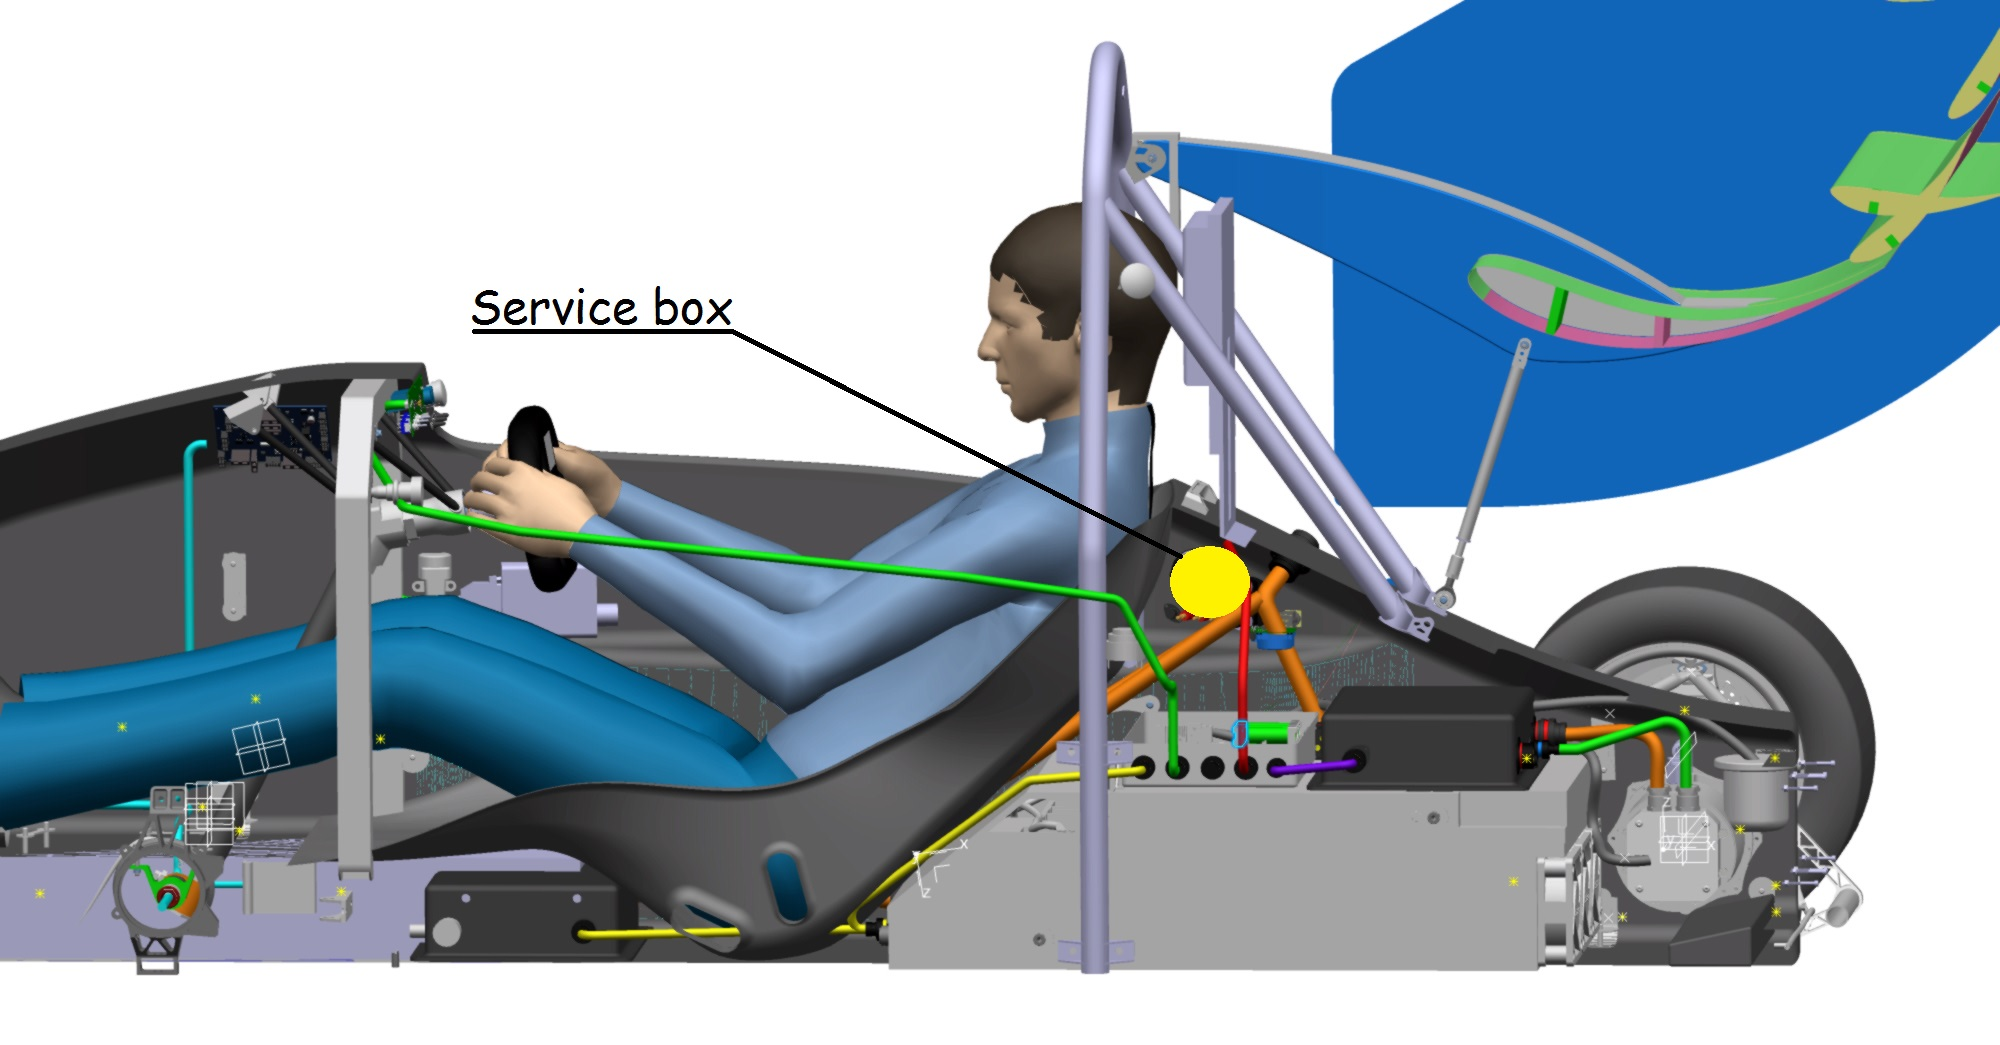
\includegraphics[width=\textwidth]{./img/ServiceBox-position.jpg}
	\caption{\gls{bspd} position}
	\label{fig:BSPD-position}
\end{figure}


\subsection{Reset / Latching for IMD and BMS} \label{subsec:Reset}
% Responsible: Kdokoliv
% ECUB scheme and circuitry, state machine and other
\subsubsection{Description/circuitry}
% Describe the concept and circuitry of the latching/reset system for a tripped IMD or AMS.  Describe the method for resetting the IMD and AMS.

\subsubsection{Wiring/cables/connectors}
\iffalse Describe wiring, show schematics, describe connectors and cables used and show useful data regarding the wiring.  If not detailed in section 2.1, be sure to show how the device opens the shutdown circuit.\fi
% SDC monitoring scheme 
Measuring, what was original problem, is done by two optocouplers in \gls{ecub}. \ref{fig:SDC-schematic}- Example of used \gls{sdc} monitoring with optocouplers.
\subsubsection{Position in car}
%Provide CAD-renderings showing the relevant parts. Mark the parts in the rendering, if necessary.
Latch as well as reset of \gls{imd} and \gls{bms} error is placed in \gls{ecub}box on the back of car. See \ref{fig:ecub_position}.

\begin{figure}[H]
	\centering
	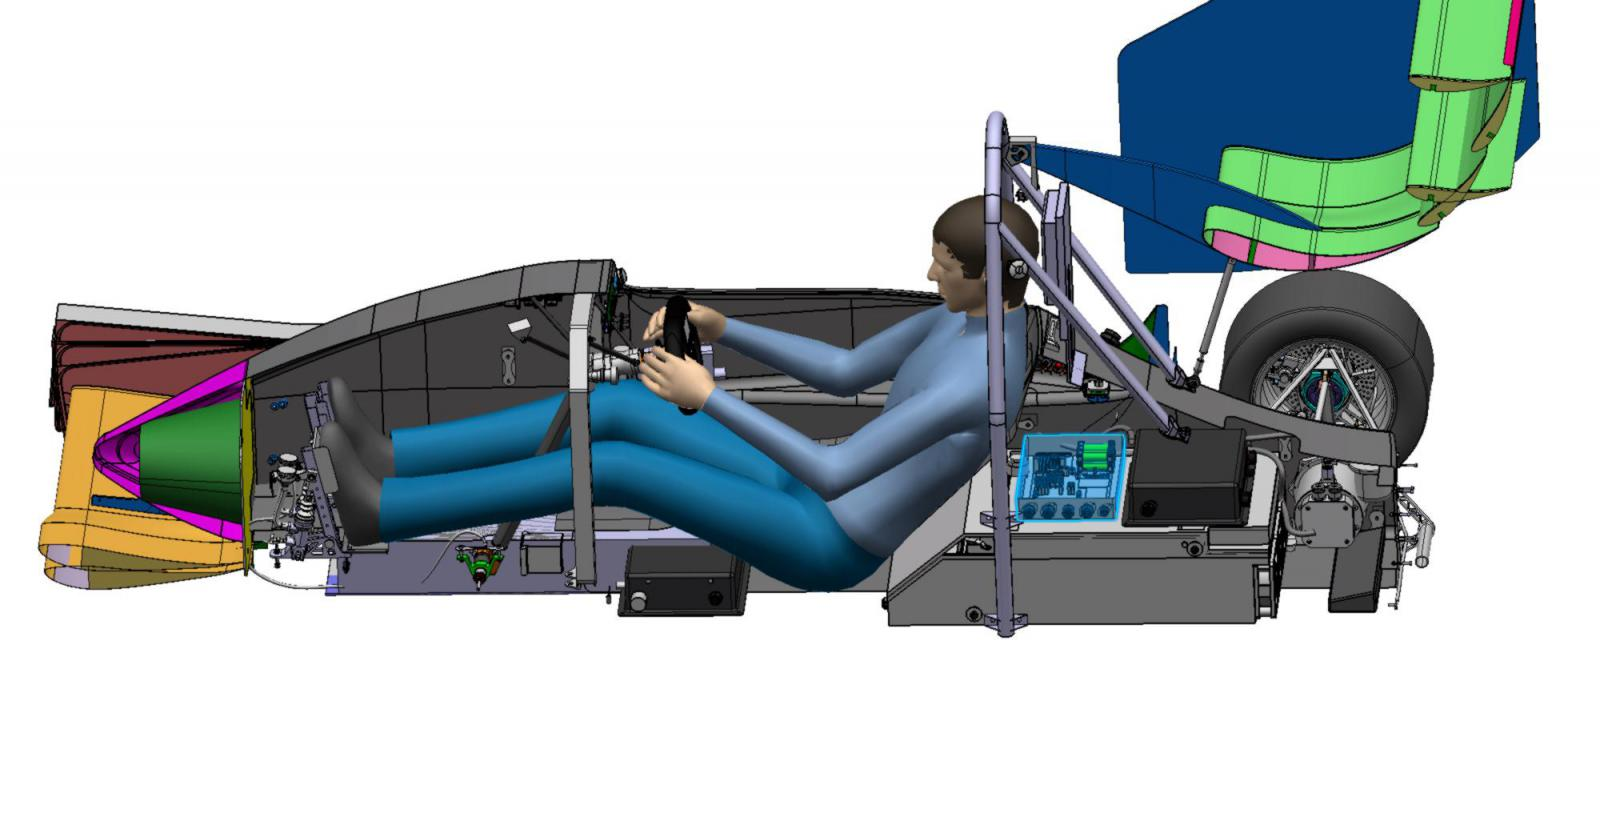
\includegraphics[width=\textwidth]{./img/ECUB_POSITION.jpg}
	\caption{\gls{bspd} schematic sheet}
	\label{fig:ecub_position}
\end{figure}

\subsection{Shutdown System Interlocks}\label{subsec:SDCInterlocks}
% figures and renderings 
%Responsible: Jano
\subsubsection{Description/circuitry}
\iffalse Describe the concept and circuitry of the Shutdown System Interlocks.
Note: Interlocks are circuits used to open the shutdown circuit if a connector is disconnected or enclosure is opened.  This is not the entire shutdown circuit.\fi

We have interlocks in ACP HV connector (connector HV\_A), Motor controller HV inputs and outputs, HV connector in Service box, HVD and in the LV connectors from ECUM´s (ECUM Rear and ECUM Front) to motor (connectors M1, M2, M3 and M4). 


In the M1-4 connectors we have a loop, that in case of disconection from car opens Shutdown circuit.
%\todo[inline]{^^ WTF?? motory to nijak nechrani...}

\subsubsection{Wiring/cables/connectors}
%Describe wiring, show schematics, describe connectors and cables used and show useful data regarding the wiring.

Scheme of entire Shutdown circuit can be found at \ref{fig:SDC-scheme}.

\subsubsection{Position in car}
%Provide CAD-renderings showing the relevant parts. Mark the parts in the rendering, if necessary.
HVD is clearly shown above in Figure 8 - Inertia switch, SDB Left, Right and Cockpit, TSMS, GLVMS, HVD, Measure points. For Service box position see Figure 17 - Motor controllers

Last interlock is in Accumulator Pack HV Connector shown in ACP HV Connector.

\subsection{Tractive System Active Light}\label{subsec:TSAL}
% Responsible: Janko, Emil, Manek
%ECUB, schemata tsal + schema v ecub + schemes + renders
\subsubsection{Description / circuitry}
% Describe the tractive system active light and additional circuitry. Additionally, fill out the table:

The \gls{tsal} is a distributed system consisting of the following components:
\begin{itemize}
\item Tractive System Active Light mounted on main hoop
\item \gls{tsal} logic \& power circuitry (located in \gls{ecub}; LV only)
\item DC-DC converter to power the \gls{tsal} in case of charged TS but unpowered \gls{glvs} (located in the \gls{acp}; has a \gls{hv} side and a LV side)
\end{itemize}

\paragraph{Tractive System Active Light}

The \gls{tsal} proper is connected with 2 wires. When voltage of 24 V is applied, the \gls{tsal} lights up either in green or red color depending on the polarity.

\begin{figure}[H]
	\centering
	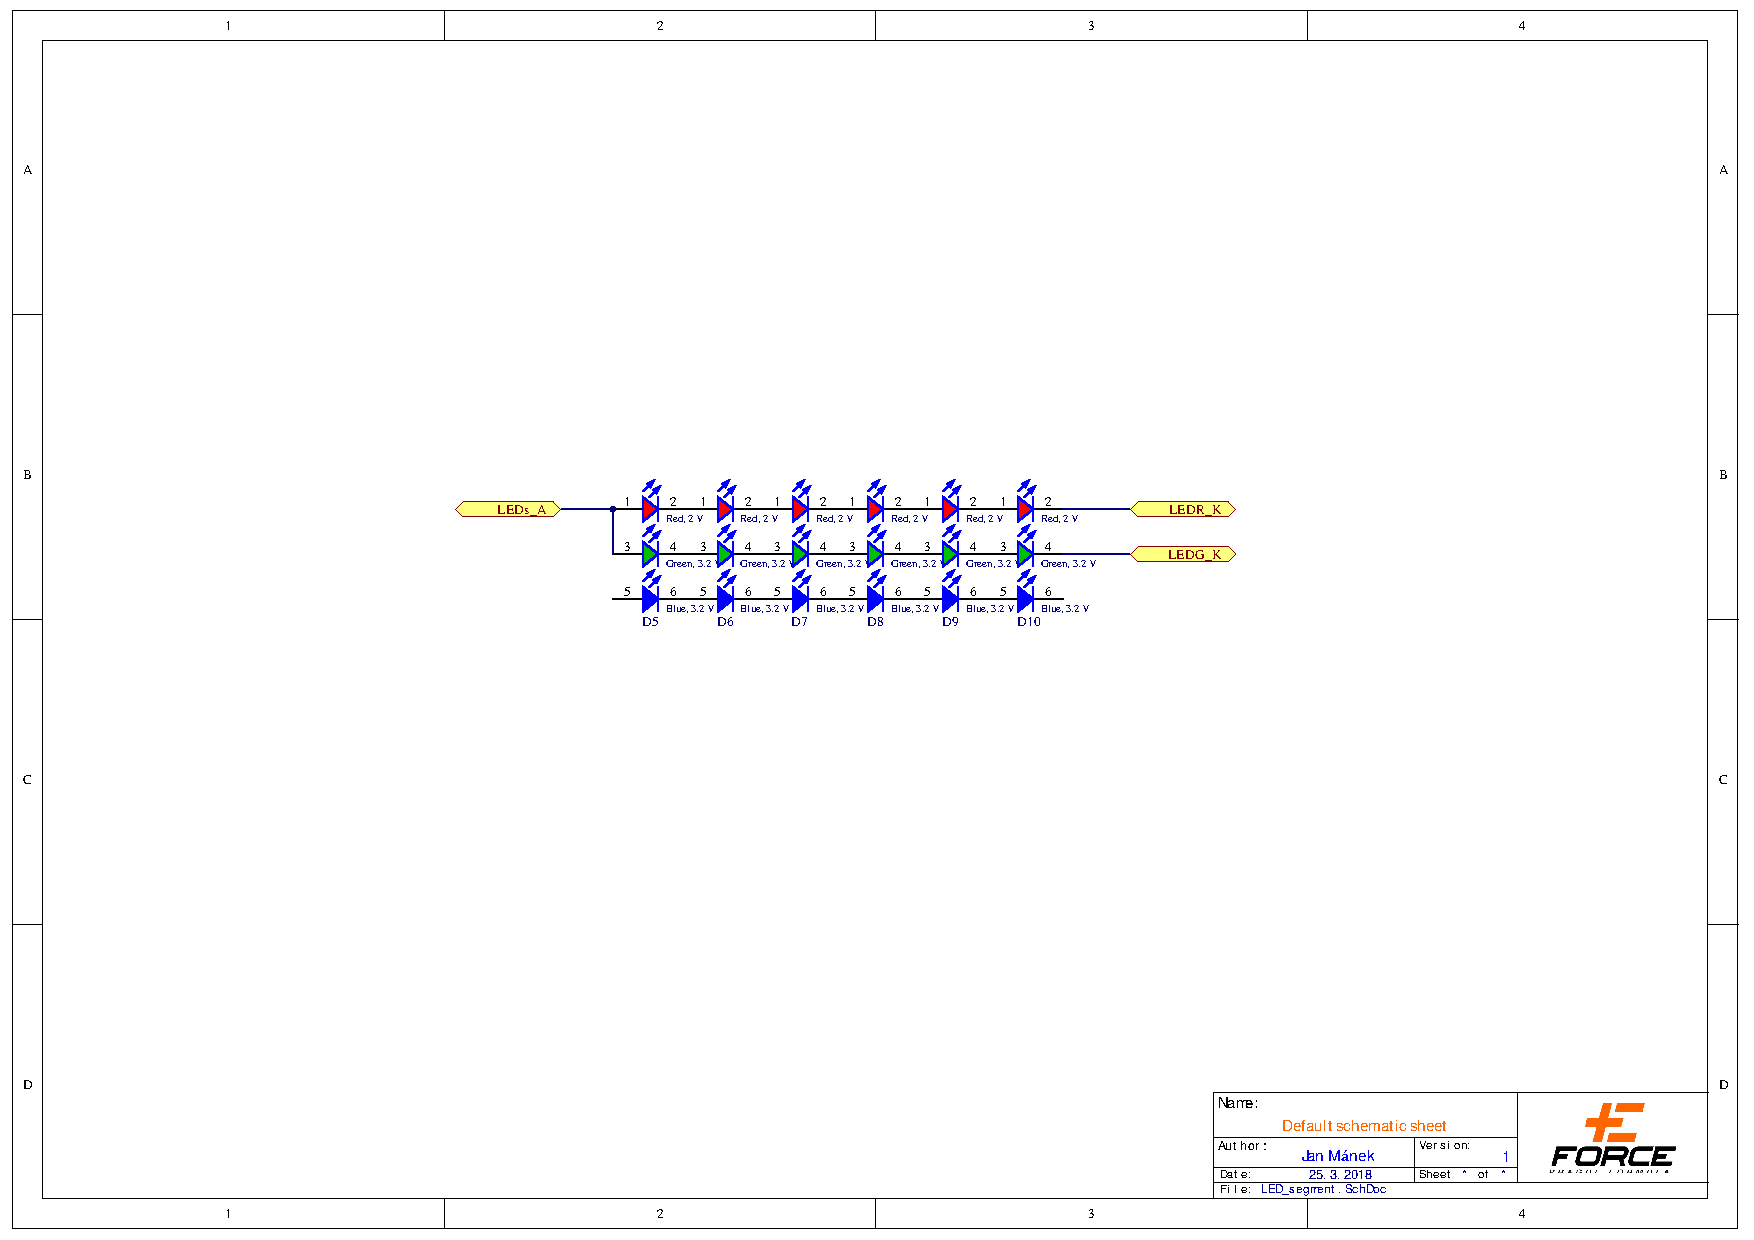
\includegraphics[width=\textwidth,trim={6cm 10cm 6cm 7cm},clip]{./img/TSAL-schematic.pdf}
	\caption{TSAL schematic.}
	\label{fig:TSAL-schematic}
\end{figure}


\begin{table}[H]
	\centering
	\caption{Parameters of the TSAL}
	\begin{tabularx}{\textwidth}{|X|X|}
		\hline
		Supply voltage: & +/- 24 V$_{DC}$ \\[\TableSize]
		\hline
		Max. operational current: & 300 mA \\[\TableSize]
		\hline
		Lamp type & Bi-color LED \\[\TableSize]
		\hline
		Power consumption: & 7.2 W \\[\TableSize]
		\hline
		Brightness & 124 Lumen (red), 29 Lumen (green) \\[\TableSize]
		\hline
		Frequency: & 3.96 Hz \\[\TableSize]
		\hline
		Size (length x height x width): & 128 mm x 20 mm x 32 mm \\[\TableSize]
		\hline
	\end{tabularx}%
	\label{tab:TSAL}%
\end{table}%

\paragraph{TSAL logic \& power circuitry}

To power the \gls{tsal}, a voltage of approximately 24 V is needed. This can be supplied either by the \gls{glvs}, or by a charged Tractive System by means of an isolated DC-DC converter.

A 5V rail is also generated to control all \gls{tsal} related logic. (\ref{fig:TSAL-ECUB-5V})

\begin{figure}[H]
	\centering
	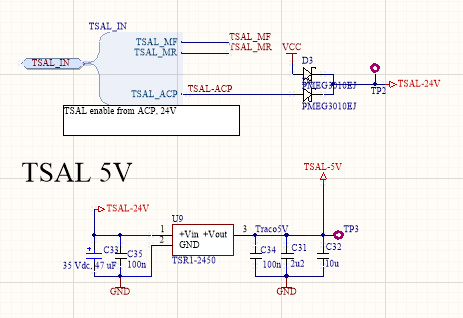
\includegraphics[width=0.6\textwidth]{./img/TSAL-ECUB-5V.png}
	\caption[Powering of the TSAL]{Powering of the \gls{tsal}. \gls{glvs} power is denoted \texttt{VCC}.}
	\label{fig:TSAL-ECUB-5V}
\end{figure}

Discrete logic is used for selecting the light colour. (\ref{fig:TSAL-logic})

\begin{figure}[H]
	\centering
	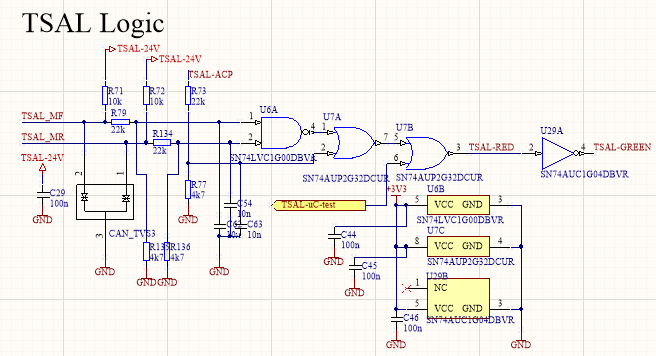
\includegraphics[width=\textwidth]{./img/TSAL-logic.png}
	\caption[TSAL enable logic]{TSAL enable logic. The signals \texttt{TSAL-RED} and \texttt{TSAL-GREEN} are always complementary.}
	\label{fig:TSAL-logic}
\end{figure}

A 555 IC is used to generate the required frequency which is used to modulate the power output. (\ref{fig:TSAL-555})

\begin{figure}[H]
	\centering
	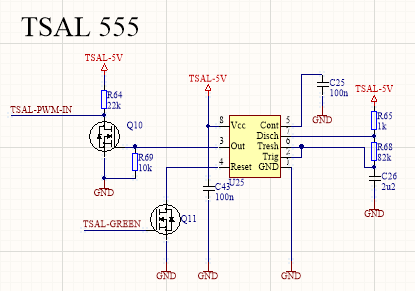
\includegraphics[width=0.6\textwidth]{./img/TSAL-555.png}
	\caption[TSAL frequency generator]{\gls{tsal} frequency generator. When a green light is desired (\gls{glvs} active, \gls{ts} not charged), oscillation is suppressed and the output \texttt{TSAL-PWM-IN} is a constant logical '1'.}
	\label{fig:TSAL-555}
\end{figure}

Finally, a H-bridge is used to drive the proper power outputs with switchable polarity. (\ref{fig:TSAL-H-bridge})

\begin{figure}[H]
	\centering
	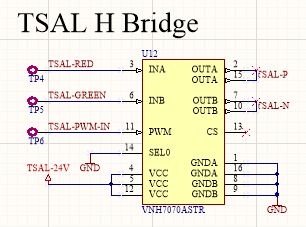
\includegraphics[width=0.5\textwidth]{./img/TSAL-H-bridge.png}
	\caption{\gls{tsal} power H-bridge}
	\label{fig:TSAL-H-bridge}
\end{figure}

\ref{fig:TSAL-logic-table} summarizes operation of the \gls{tsal}.

\begin{table}[H]
	\centering
	\caption{TSAL logic table}
	\begin{tabularx}{\textwidth}{|X|X|X|X|X|}
		\hline
		\textbf{Tractive System state} & \textbf{GLVS state} & \textbf{TSAL powered from} & \textbf{TSAL polarity} & \textbf{TSAL waveform} \\
		\hline
		not charged & off & not powered & -- & -- \\
		\hline
		not charged & on & 24 V GLVS & negative (green) & Always-on \\
		\hline
		precharging & on & 24 V GLVS & positive (red) & Square wave, 3.96 Hz, 50\% duty cycle \\
		\hline
		charged & don't care & TS & positive (red) & Square wave, 3.96 Hz, 50\% duty cycle \\
		\hline
	\end{tabularx}%
	\label{fig:TSAL-logic-table}
\end{table}%

\paragraph{DC-DC converter}

To ensure that the \gls{tsal} continues to operate even after disabling \gls{glvs}, the following circuit is used:

\begin{figure}[H]
	\centering
	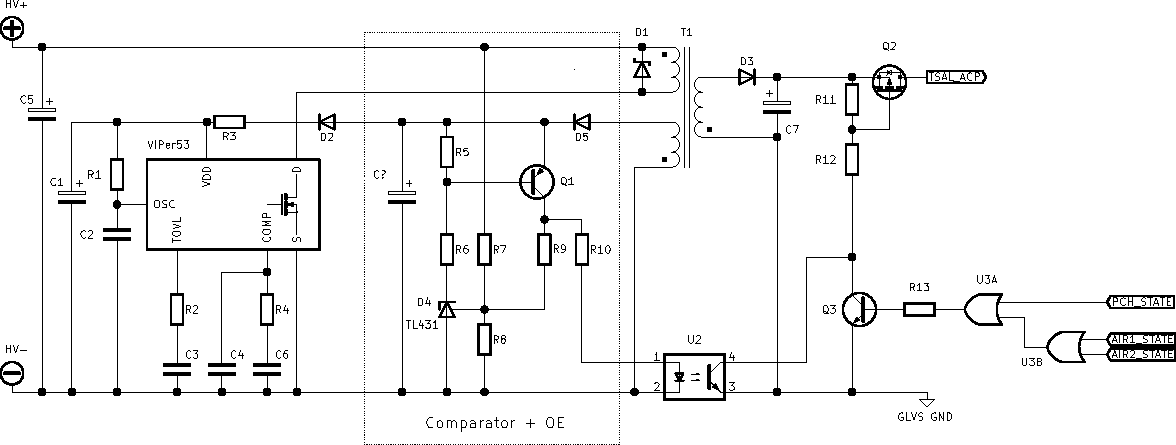
\includegraphics[width=\textwidth]{./img/ECUA_TSAL_POWER.pdf}
	\caption{TSAL HV part schematic.}
	\label{fig:TSAL-HV}
\end{figure}

\paragraph{Explanation of TSAL circuit}
\Gls{tsal} \gls{hv} part schematic \ref{fig:TSAL-HV} is directly connected to the output \gls{hv} pins of \gls{acp}. The circuit is designed with STMicroelectronics chip VIPer53 (\ref{app:viper_datasheet}). The circuit functions as a fly-back DC/DC converter, directly supplying the \gls{tsal}. The converter starts operating at about 40 V, but the output to \gls{tsal} is switched through $Q_2$ only when the HV voltage is more than 60 V. That is ensured using D4, which together with $Q_1$ works as a precise 60 V comparator with a little introduced hysteresis.

The \gls{acp} indication led is powered from the primary side of the transformer, from the VIPER53's own supply voltage.
In case of any of the \glspl{air} closed, or the pre-charge relay contact being detected closed (please see \ref{subsec:precharge}  for details), the \gls{tsal} is supplied from the \gls{glvs} 24 V system, through Q$_2$. The "relay closed" signals from both \glspl{air} and the pre-charge relay are OR-ed together using hardwired logic (i.e. 74LVC2G32).

%schema z backu
\subsubsection{Wiring/cables/connectors}
\iffalse Describe wiring, show schematics, describe connectors and cables used and show useful data regarding the wiring.  Include gauge, voltage and temperature rating of wiring used and any fuses or other overcurrent protection used.\fi

LEDs are supplied from \gls{ecub} (by Harness\_D by connector D1) by 2-wire low voltage cable (\ref{fig:TSAL-wiring}).

\begin{figure}[H]
	\centering
	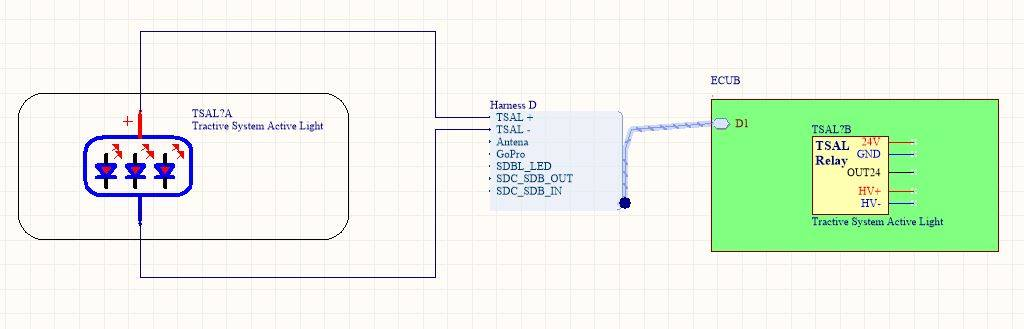
\includegraphics[width=\textwidth,]{./img/tsal-wiring.jpg}
	\caption{Wiring \gls{tsal} from \gls{ecub}}
	\label{fig:TSAL-wiring}
\end{figure}

\subsubsection{Position in car}
%Provide CAD-renderings showing the relevant parts. Mark the parts in the rendering, if necessary.
\gls{tsal} is placed under the main roll hoop, see \ref{fig:TSAL-position}

\begin{figure}[H]
	\centering
	\includegraphics[width=\textwidth,trim={3cm 11cm 2cm 1cm},clip]{./img/tsal-position.pdf}
	\caption{\Gls{tsal} position.}
	\label{fig:TSAL-position}
\end{figure}

\begin{figure}[H]
	\centering
	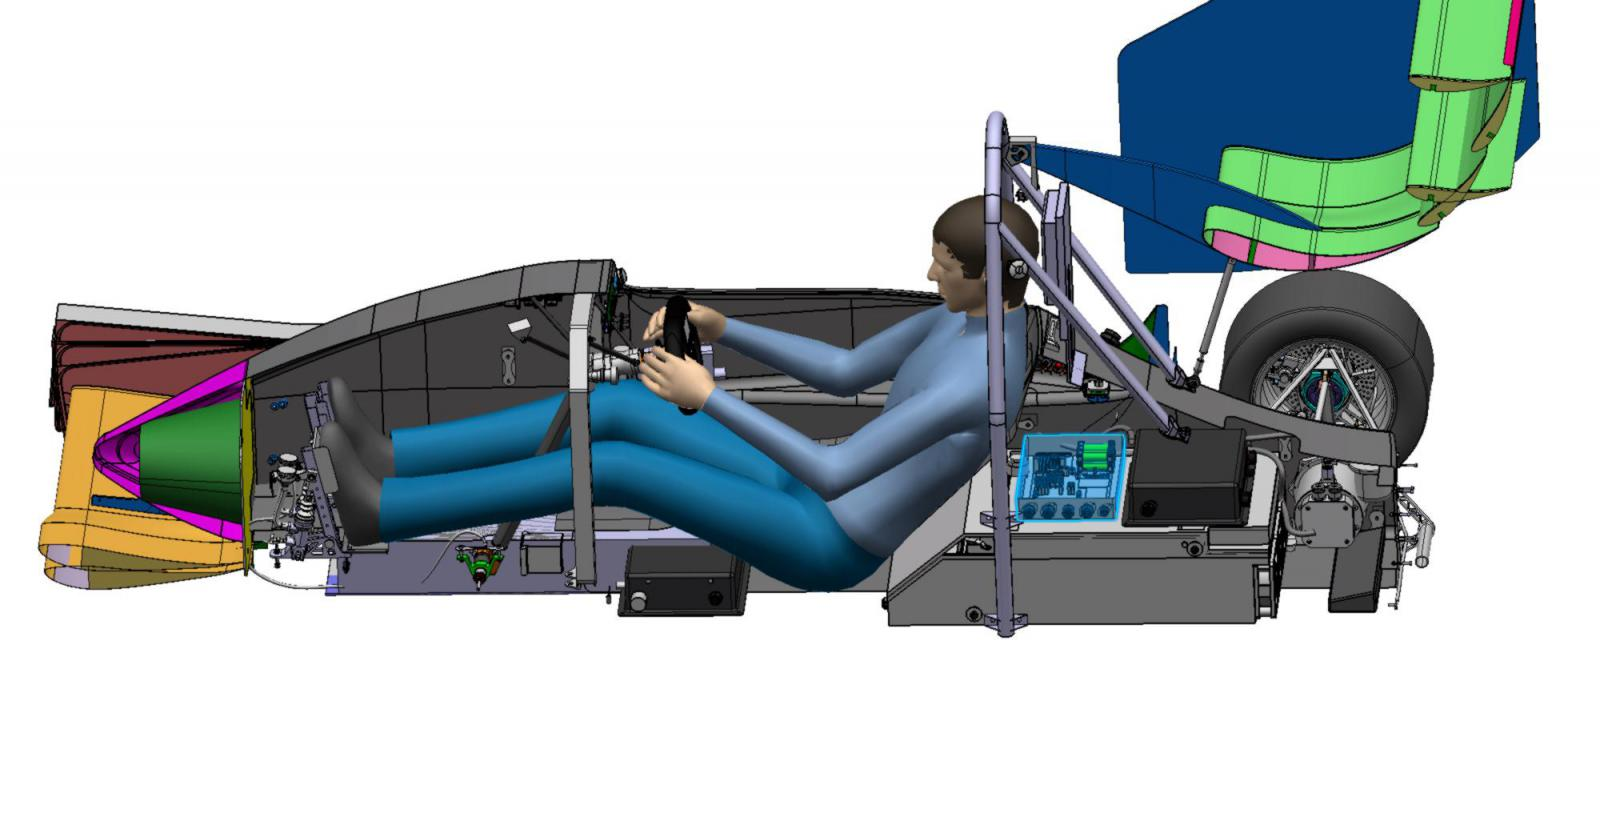
\includegraphics[width=\textwidth]{./img/ECUB_POSITION.jpg}
	\caption{\gls{bspd} schematic sheet}
	\label{fig:ecub_position}
\end{figure}


\subsection{Measurement points}\label{subsec:MeasurementPoints}
%Responsible: Janko
%schemata
\subsubsection{Description}
%Describe the housing used and how it can be accessed, etc.  Describe how the measurement points protected/covered when not in use and how the electrical connections on the back of the measurement points are protected when the measurement points are being used.

High voltage measurement points (HVMP) are placed in the Service box. When not in use, they are covered with protective cups made from silicone rubber. From backside they are protected by heat shrink tube, which prevents moisture from getting in and also accidental touching of high voltage poles.

\subsubsection{Wiring, connectors, cables}
%Describe wiring, show schematics, and describe connectors and cables used and show useful data regarding the wiring.  Include details on the protection resistor including resistance, voltage and power rating.

HVMP wires will be connected to the Service box, where are terminals connecting Accumulator to Motor controller. There are also 2 resistors 10k 5W (R1, R2) wired between those 2 terminals and HVMP. Value of this resistor can be measured from measuring points by multimeter with switched TSMS off. Service box scheme is shown in \ref{fig:ServiceBox/scheme}.

\begin{figure}[H]
	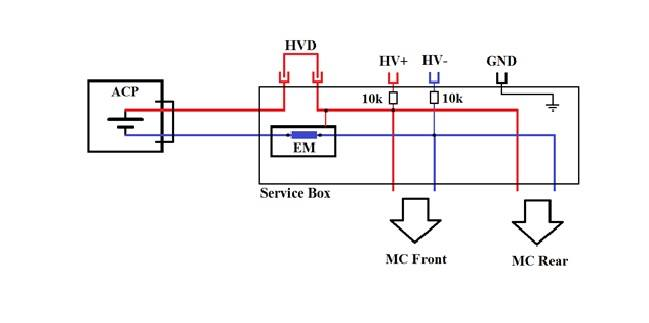
\includegraphics[width=\textwidth]{./img/ServiceBox-scheme.jpg}
	\caption{Service box scheme}
	\label{fig:ServiceBox/scheme}
\end{figure}

\subsubsection{Position in car}
%Provide CAD-renderings showing the relevant parts. Mark the parts in the rendering, if necessary.

Measure points are placed on panel next to Master switches and HVD, see \ref{fig:SDC-positionInCar}.

\subsection{Pre-Charge circuitry}\label{subsec:PrechargeCircuitry}
%Responsible: JSi
%ECUA
\subsubsection{Description}

\begin{figure}[H]
	\centering
	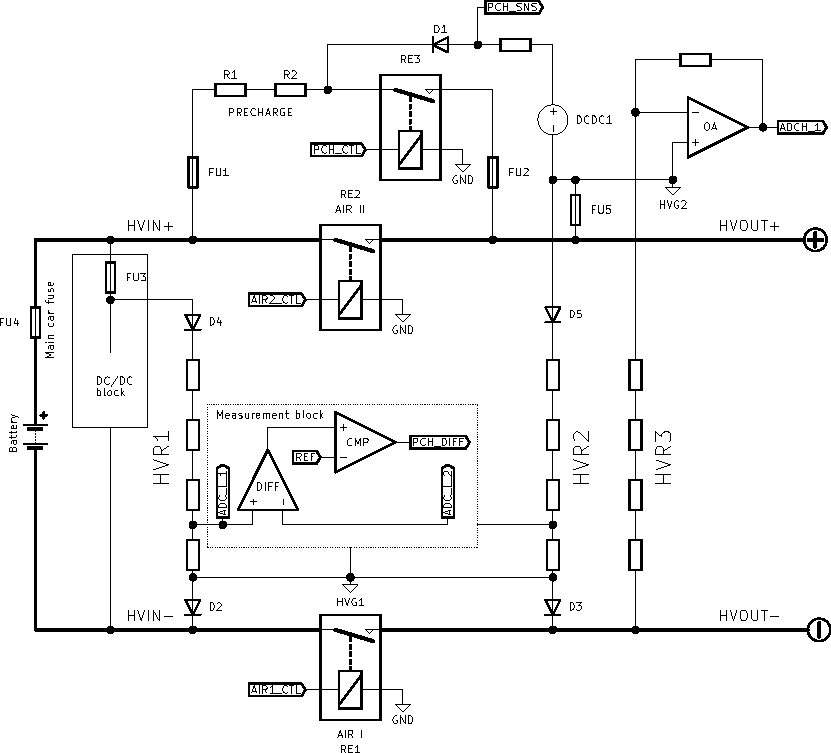
\includegraphics[width=\textwidth,clip]{./img/ECUA_AIRS.pdf}
	\caption{TS pre-charge circuit and switching schematic.}
	\label{fig:precharge_sch}
\end{figure}

Principial block schematic of the TS switching circuit (including pre-charge) is in the \ref{fig:precharge_sch}. Pre-charge circuit is part of and controlled by \gls{ecua}. Pre-charge circuit is comprised of a relay RE$_3$ and two series connected power resistors R$_1$ and R$_2$. 

Both resistors are located on a heat-sink, that is shared with the DC/DC converters, mentioned in \ref{subsec:glvs_dcdc} of this document. The task of the heat-sink is to enhance the power overload capacity of the pre-charge resistors during the initial overload during the beginning of the charging curve, shown in \ref{fig:precharge_voltage_time}.

\begin{figure}
	\begin{tikzpicture}
		\begin{axis}[
			use units,
			x unit=s,
			y unit=V,
			xlabel=time,
			ylabel=volatge,
			width=0.9\textwidth,
			height=0.5\textwidth,
			grid=major,
			xmin=0,
			ymin=0,
			xmax=10
			]
		\addplot[red, smooth] table[
			x=time,
			y=voltage,
			col sep=comma
			] {./data/TS_precharge.csv};
		\end{axis}
		\end{tikzpicture}
		\caption{Pre-charge voltage in time.}
	\label{fig:precharge_voltage_time}
\end{figure}

The formula describing \ref{fig:precharge_voltage_time} is:

\begin{equation}
	V_{c}=V_{s}*(1-e^{(\frac{-t}{R*C})})
	\label{eq:precharge_voltage}
\end{equation}

\begin{figure}
	\begin{tikzpicture}
	\begin{axis}[
	use units,
	x unit=s,
	y unit=A,
	xlabel=time,
	ylabel=current,
	width=0.9\textwidth,
	height=0.5\textwidth,
	grid=major,
	xmin=0,
	ymin=0,
	xmax=10
	]
	\addplot[red, smooth] table[
	x=time,
	y=current,
	col sep=comma
	] {./data/TS_precharge.csv}; 
	\end{axis}
	\end{tikzpicture}
	\caption{Precharge current in time.}
	\label{fig:precharge_current_time}
\end{figure}

The formula describing \ref{fig:precharge_current_time} is:

\begin{equation}
	I=\frac{V_{c}-V_{s}}{R}	
	\label{eq:precharge_current}
\end{equation}


Both wirewound power resistors, ARCOL HS25 series, have 250 $\Omega$, 25 W continuous rating, (\ref{app:precharge_resistors}).

All three TS relays RE$_1$ to RE$_3$ coils are powered directly from the \gls{sdc} end.

After the \gls{sdc} circuit is complete and closed (voltage present at \gls{sdc} END), the pre-charge sequence is begun by closing AIR I (RE$_1$). Then a pre-charge relay RE$_3$ is closed. Voltage both on the \gls{acp} and output side is monitored using the measurement block, through the $HVR_1$ and HVR$_2$ resistor dividers. After the voltage difference is low enough (determined by \gls{ecua} software), AIR II (RE$_2$) is closed, RE$_3$ can be released.

Safety of the AIR switching and pre-charging is done by the \gls{ecua} firmware, that evaluates all possible circuit states. Voltages are measured on the \gls{acp} and \gls{acp} output sides using the measurement block, AIR physical states are observed using the auxiliary contacts and the pre-charge relay physical contact state is observed using the principle in the \ref{fig:precharge_sch}, via the diode D$_1$. The PCH\_SNS signal is pulled low whenever the pre-charge relay RE$_3$ contact is closed.

Several safety precautions are implemented, on top of the Rules. First of such implemented protections is HW non-programmable voltage difference sensing across the pre-charge relay or AIR II respectively. This is done using the two voltage measurement dividers HVR$_1$ and HVR$_2$. There is a differential amplifier and comparator, that prevents closing both AIR relays in case of high voltage difference across the AIR II. 

Diodes D$_2$ and D$_3$ serve to block current flow to the output in case of AIR I is open. This specific topology was chosen to be able to measure the difference voltage across the AIR II utilizing only analog non-programmable circuitry.

Second precaution is a \gls{hv} circuit limiting the maximum pre-charge relay closed time, and assuring a minimum off time for the pre-charge resistor to cool off. This circuit is a non-programmable one, realized using a discrete logic. In case of a pre-charge time-out or failure (voltages not equalized), AIR I (the Tyco Kilovac EV200 \ref{app:air_datasheet}) is disconnected always first (instead of the pre-charge relay RE$_3$), because the \gls{air} does have the required DC breaking capacity.

Additional precision \gls{acp} voltage measurement is taken using the HVR$_3$ sense divider, as this measurement is not influenced by the forward voltage drops of diodes D$_2$ to D$_5$. This measurement together with the measured \gls{acp} current serves to calculate power drawn from the \gls{acp}. This measurement is then presented on the \gls{can} bus for other car \glspl{ecu}, for example to estimate the SOC, instantenous power, etc.  

The TS voltage sensing dividers HVR$_1$, HVR$_2$ and HVR$_3$ are realized with a high voltage 3500 V rated resistors from Vishay, HVR$_{37}$ series (\ref{app:hvr37_datasheet}). All dividers use 10 M$\Omega$ resistors as the top side of the divider. All diodes D$_1$ to D$_5$ are SM4007 (DATASHEET) or equivalent type, 1000 V rated. The blocking voltage is therefore sufficient to safely withstand the maximum \gls{acp} voltage of 400 V.

\paragraph{Pre-charge safety on \gls{ecua}}
Except from what rules require we implemented several safety precautions. In case, that \gls{sdc} error doesn’t occur and driver pushed TS ON button following safety precautions are taken to prevent switching AIR in case of problem that has not yet been detected.

First one is completely non-programmable protection against switching voltage difference by \gls{air}. It uses voltage measurement and then comparators and logic to disable \gls{mcu} decision in case of SW error.
Second one is measuring all states and voltages by \gls{mcu} on \gls{ecua} which can determinate error before non-programmable protection would have to act.

Third (time-out) protection is used when everything seems to be OK, but the charging is too slow – caused by too high pre-charge resistance (any of pre-charge resistors fails), or some leakage of charge in capacitor or any other possible error occurs. If voltage difference is not equaled in time less them 2seconds, the \gls{ecua} stops pre-charge and waits 5 seconds before trying again. (In order to not overpower resistors.) If number of attempts to pre-charge is in this state higher then 8, something is clearly wrong and \gls{ecua} opens \gls{sdc} and indicates error. Sending message about error and sets car into not-ready state.

\subsubsection{Wiring, cables, current calculations, connectors}
%Describe wiring, show schematics, describe connectors and cables used and show useful data regarding the wiring.

%\item Give a plot “Percentage of Maximum Voltage” vs. time
%\item Give a plot Current vs. time 
%\item For each plot, give the basic formula describing the plots
There is no connectors nor cables it is realised on PCB in ECUA. 

%Additionally, fill out the tables:

\begin{table}[H]
	\centering
	\caption{General data of the pre-charge resistor}
	\begin{tabularx}{\textwidth}{|X|X|}
		\hline
		Resistor Type: & NTC \\[\TableSize]
		\hline

		Resistance: & 25 $\Omega$ at 25 $^\circ$C\\[\TableSize]
		\hline
		Continuous power rating: & 25 W \\[\TableSize]
		\hline
		Overload power rating (1 sec): & not specified \\[\TableSize]
		\hline
		Overload power rating (5 sec): & not specified \\[\TableSize]
		\hline
		Overload power rating (15 sec): & not specified \\[\TableSize]
		\hline
		Voltage rating: & 680 V$\_AC$\\[\TableSize]
		\hline
		Cross-sectional area of the wire used: & 0.195 mm$^2$\\[\TableSize]
		\hline
	\end{tabularx}%
	\label{tab:precharge-general}%
\end{table}%

\begin{table}[H]
	\centering
	\caption{General data of the pre-charge relay}
	\begin{tabularx}{\textwidth}{|X|X|}
		\hline
		Relay Type: & Finder 40.52\\[\TableSize]
		\hline
		Contact arrangement: &  SPDT \\[\TableSize]
		\hline
		Continuous DC current:  & 10 A\\[\TableSize]
		\hline
		Voltage rating  & 400 V\\[\TableSize]
		\hline
		Nominal Coil Voltage: & 24 V \\[\TableSize]
		\hline
		Cross-sectional area of the wire used: & 0.195 mm$^2$ \\[\TableSize]
		\hline
	\end{tabularx}%
	\label{tab:precharge-relay}%
\end{table}%
\todo[inline]{civka 24 V?}

\subsubsection{Position in car}
%Provide CAD-renderings showing all relevant parts. Mark the parts in the rendering, if necessary.

\begin{figure}[H]
	\centering
	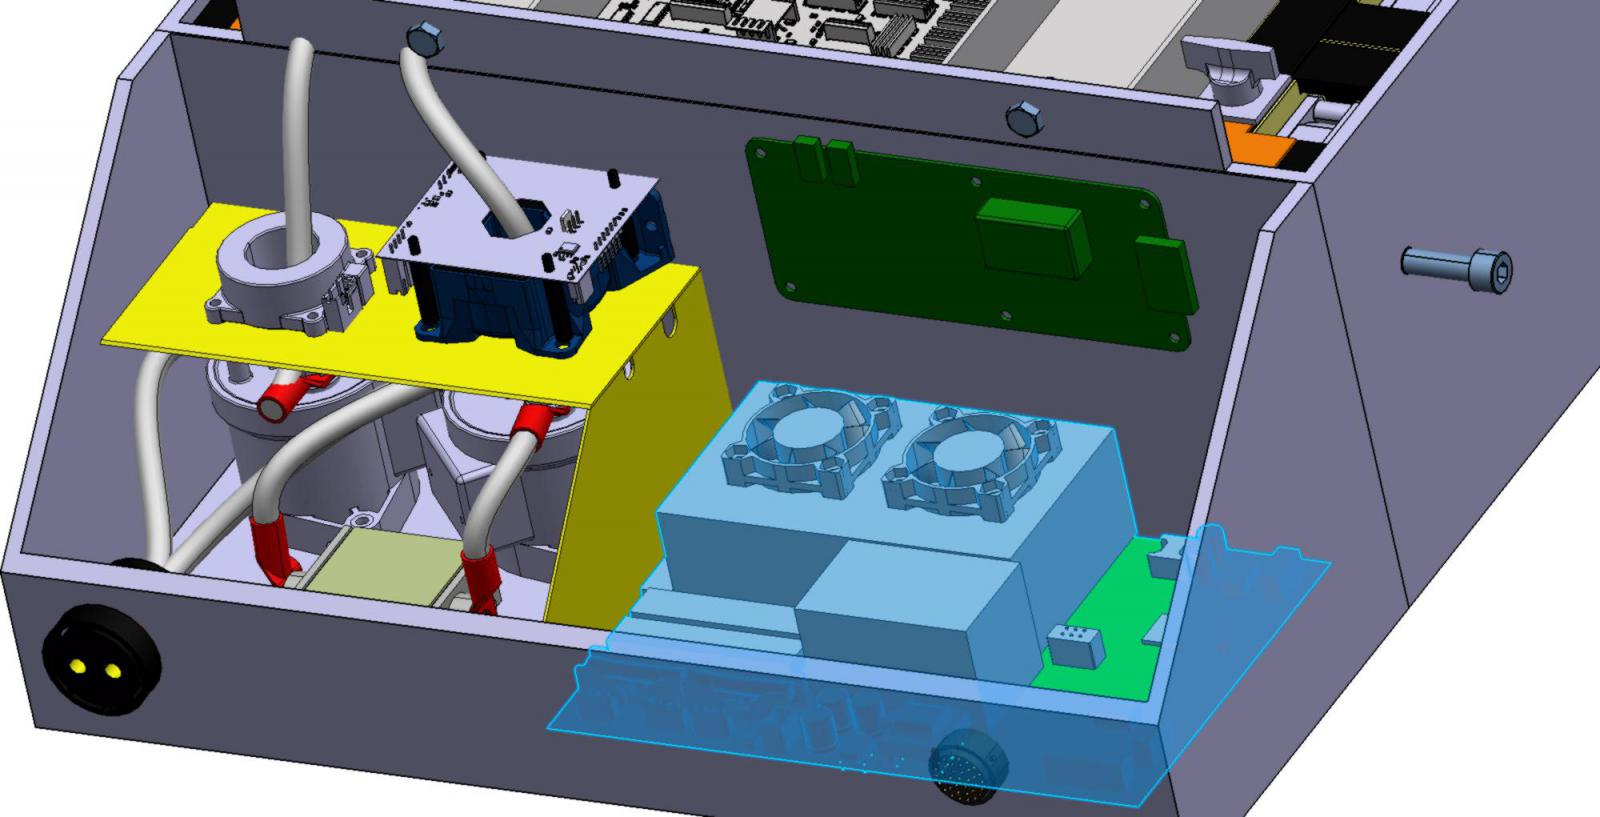
\includegraphics[width=\textwidth]{./img/ECUA_POSITION.jpg}
	\caption{ECUA position.}
	\label{fig:ECUA}
\end{figure}

\subsection{Discharge circuitry}\label{subsec:DischargeCircuitry}
%ECUB
\subsubsection{Description}
%Describe your concept of the discharge circuitry.

Discharge circuit's purpose is to discharge capacities connected to \gls{ts} and ensure \gls{ts} safety in shutdown state. Such capacities are only in two \glspl{mc}.

Discharge is activated whenever \gls{sdc} is open. (That means, \gls{acp} is disconnected from \gls{ts} by\glspl{air}). This behavior is controlled by signal from \gls{ecua} which activates discharge if low \gls{air} is open. Discharge can be forced on (bot not off) by request through CAN. 

In case of \gls{glvs} power loss, discharge relays immediately close (powered from \gls{glvs}, normally closed contact) and activate discharge circuitry.

\subsubsection{Wiring, cables, current calculations, connectors}
%\iffalse Describe wiring, show schematics, describe connectors and cables used and show useful data regarding the wiring.
%\begin{itemize}
	%	\item 	Give a plot “Voltage” vs. time 
	%	\item 	Give the formula describing this behavior
	%	\item 	Give a plot “Discharge current” vs. time
	%	\item 	Give the formula describing your plot
%\end{itemize}\fi

\begin{figure}[H]
	\centering
	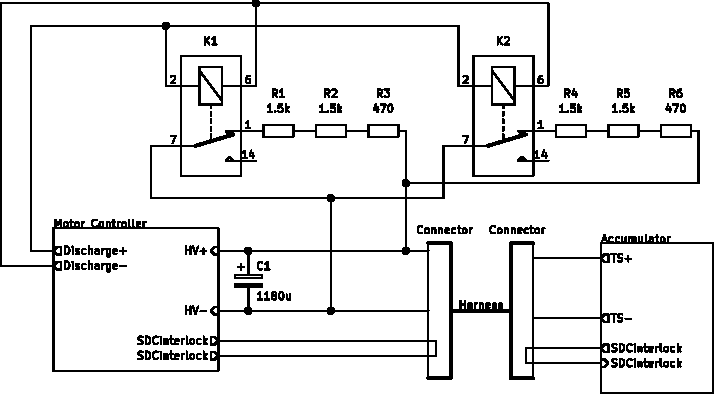
\includegraphics[width=0.7\textwidth]{./img/MC_discharge.pdf}
	\caption{Discharge circuit of one \gls{mc}. (two present in car)}
	\label{fig:discharge-circuit}
\end{figure}

\ref{fig:discharge-circuit} shows a simplified discharge circuitry. Discharge resistors are placed in \glspl{mc} right next to the only capacity that provides a storage for potentially dangerous charge/energy in \gls{ts}. If \gls{hv} cable is disconnected on either side, the \gls{sdc} opens due to the interlocks and both \glspl{air} open. Because there is no output capacitance in \gls{acp} there is no way the power could be on \gls{acp} output \gls{hv} connector.

Capacity sum of all capacitors in \glspl{mc} is 2360 $\mu$F. For discharging this capacity in less than 5 seconds to voltage (below 60 V), maximum resistor value is calculated by solving R from \ref{eq:discharge_voltage_eq}.

\begin{equation}
	V_{c}=V_{s}*e^{(\frac{-t}{R*C})}
	\label{eq:discharge_voltage_eq}
\end{equation}

\paragraph{Values}
\begin{itemize}
	\item V$_c$ = 60 V (safe voltage limit)
	\item V$_s$ = 400 V (\gls{ts} voltage)
	\item t = 5 s (maximum discharge time)
	\item C = 2360 $\mu$F (total capacity in \gls{ts})
\end{itemize}

Maximum resistance from equation \ref{eq:discharge_voltage_eq}, $R = 1112\Omega$ is for discharging all capacitors in \gls{ts}. In our case, capacity is split between two \glspl{mc}. Two parallel resistor combinations of three 1 k\ohm resistors in series (3s2p) in each \gls{mc} is used (3s4p in total). 1 k\ohm resistors are PWR221T-30-1001F. Total value of Discharge resistor bank is R = 750 \ohm, which is less than maximal calculated R = 1112 \ohm. The 60V threshold with such configuration is reached in $3.37s$. \ref{fig:discharge_voltage_time} shows \gls{ts} voltage in time during discharging.

\begin{figure}
	\begin{tikzpicture}
		\begin{axis}[
			use units,
			x unit=s,
			y unit=V,
			xlabel=time,
			ylabel=voltage,
			width=0.9\textwidth,
			height=0.5\textwidth,
			grid=major,
			xmin=0,
			ymin=0,
			xmax=20,
			ymax=410
			]
			\addplot[red, smooth] table[
				x=time,
				y=voltage,
				col sep=comma
				] {./data/TS_discharge.csv}; 
			\addplot [mark=none, black, dashed] coordinates {(0, 60) (20, 60)};
			\addplot [mark=none, black, dashed] coordinates {(5, 0) (5, 410)};
		\end{axis}
	\end{tikzpicture}
	\caption{\gls{ts} voltage during discharge. (\glspl{air} open)}
	\label{fig:discharge_voltage_time}
\end{figure}


\begin{figure}
	\begin{tikzpicture}
		\begin{axis}[
			use units,
			x unit=s,
			y unit=A,
			xlabel=time,
			ylabel=current,
			width=0.9\textwidth,
			height=0.5\textwidth,
			grid=major,
			xmin=0,
			ymin=0,
			xmax=20
			]
			\addplot[red, smooth] table[
			x=time,
			y=current,
			col sep=comma
			] {./data/TS_discharge.csv}; 
		\end{axis}
	\end{tikzpicture}
	\caption{Discharge current through resistor bank vs. time}
	\label{fig:discharge_current_time}
\end{figure}



The formula describing \ref{fig:discharge_current_time} is:

\begin{equation}
	I_{d}=\frac{V_{C}-V_{s}}{R_{d}}	
\end{equation}


Where $V_{s}$ is voltage on \gls{ts}, $R_{d}$ is total value of discharge resistor bank and $I_{d}$ is discharge current. Current through individual 3s resistor combinations can be calculated as $I_{d}$/$4$.


\begin{figure}
	\begin{tikzpicture}
		\begin{axis}[
			use units,
			x unit=s,
			y unit=W,
			xlabel=time,
			ylabel=power loss,
			width=0.9\textwidth,
			height=0.5\textwidth,
			grid=major,
			xmin=0,
			ymin=0,
			xmax=20
			]
			%\pgfplotstableread{./data/TS_discharge_current.csv}\dischargeData;
			\addplot[red, smooth] table[
				x=time,
				y expr=(\thisrow{current}/4)^2*3000,
				col sep=comma
				] {./data/TS_discharge.csv}; 
			\addlegendentry{3s resistor combination $P_{loss}$}
			\addplot[orange, smooth] table[
				x=time,
				y expr=(\thisrow{current}/4)^2*1000,
				col sep=comma
				] {./data/TS_discharge.csv};
			\addlegendentry{1 resistor $P_{loss}$}
		\end{axis}
	\end{tikzpicture}
	\caption{Discharge power loss on 3s resistor combination and individual resistors vs. time}
	\label{fig:discharge_power_time}
\end{figure}

Peak power on individual resistors is 18 W and resistor can handle up to 30 W, see \ref{app:discharge_resistor_sheet}.

\begin{table}[H]
	\centering
	\caption{General data of the discharge circuit}
	\begin{tabu}{|X|X|}
		\hline
		Resistor Type: & PWR221T-30-1001F in 3s4p configuration \\
		\hline
		Resistance: & 1 k\ohm \\
		\hline
		Continuous power rating: & 30 W \\
		\hline
		Overload power rating (1 sec): & not specified \\
		\hline
		Overload power rating (5 sec): & not specified \\
		\hline
		Overload power rating (15 sec): & not specified \\
		\hline
		Voltage rating: & 250V (3 in series: 750 V) \\
		\hline
		Maximum expected current: & 0.1 A per resistor, (3s4p configuration with total 0.4A current) \\
		\hline
		Average current: & 0.04 A through resistor(average from 4 seconds of discharging) \\
		\hline
		Cross-sectional area of the wire used: & $0.129 mm^2$ \\
		\hline
	\end{tabu}%
	\label{tab:dischrage-circ}%
\end{table}%

\begin{table}[H]
	\centering
	\caption{General data of the dis-charge relay}
	\begin{tabu}{|X|X|}
		\hline
		Relay Type: & G6A-274P-ST-US, one per 3s resistor bank (130 mA)\\
		\hline
		Contact arrangement: & DPDT \\
		\hline
		Continuous DC current: & 2 A \\
		\hline
		Voltage rating  & 220 \vdc (per contact, 2 in series) \\
		\hline
		Nominal Coil Voltage:  & 12 V\\
		\hline
		Cross-sectional area of the wire used: & 0.129 $mm^2$ \\
		\hline
	\end{tabu}%
	\label{tab:discharge-relay}%
\end{table}%

\ref{app:discharge_relay_datasheet}


\subsubsection{Position in car}
%Provide CAD-renderings showing all relevant parts. Mark the parts in the rendering, if necessary.

Discharge resistors are mounted on aluminum cooler also with IGBT modules in \gls{mc} boxes.

\subsection{HV Disconect (HVD)}\label{subsec:HVD}
%Responsible: Jano
%Datasheety, rendery
\subsubsection{Description}
%Describe your concept of the HVD and how it can be operated.

A circular connector ASHD 0 24-44420 S N + ASHD 6 24-44420 P N are used as HVD. By disconnecting HVD, positive and negative pole of Tractive System is quickly disconnected. Disconnection is done by turning the plug left, this motion is clearly hinted by a label. By turning left the lever system in connector disconnect pins and release plug. There are sockets used in the receptacle rather than pins, therefore no harm can be done to crew by touching the receptacle. 

Interlock is achieved by using ASHD 0 24-44420 S N - 016 as a receptacle and ASHD 6 24-44420 P N - 016 as plug. This connector has several other low current pins size AWG 22. Two of them are used as interlock, there is only shunt loop at the plug.

Datasheet is to be seen in \ref{app:HVD}.

\subsubsection{Wiring, cables, current calculations, connectors}
%Describe wiring, show schematics, describe connectors and cables and show useful data regarding the wiring.  Include information on the working voltage and current rating of the HVD.

HVD is placed between Accumulator Pack and Motor Controllers, Energy Meter is also placed after Motor Controller in the circuit. Positive and negative pole of Tractive system is interrupted. There are four pins connected to each other in the plug and the back of the plug is sealed. OLFLEX HEAT 180 SiF are used as HV wires. One HV pin is rated to 200A.

\subsubsection{Position in car}
%Provide CAD-renderings showing all relevant parts. Mark the parts in the rendering, if necessary.

HVD is placed on panel next to Maser switches and Measure points, see \ref{fig:hvd-position}. It is placed in rollover protection envelope, see \ref{fig:hvd2}.

\begin{figure}[H]
	\centering
	\includegraphics[width=\textwidth,trim={15cm 2cm 15cm 5cm},clip]{./img/hvd-position.jpg}
	\caption{HVD position.}
	\label{fig:hvd-position}
\end{figure}

\begin{figure}[H]
	\centering
	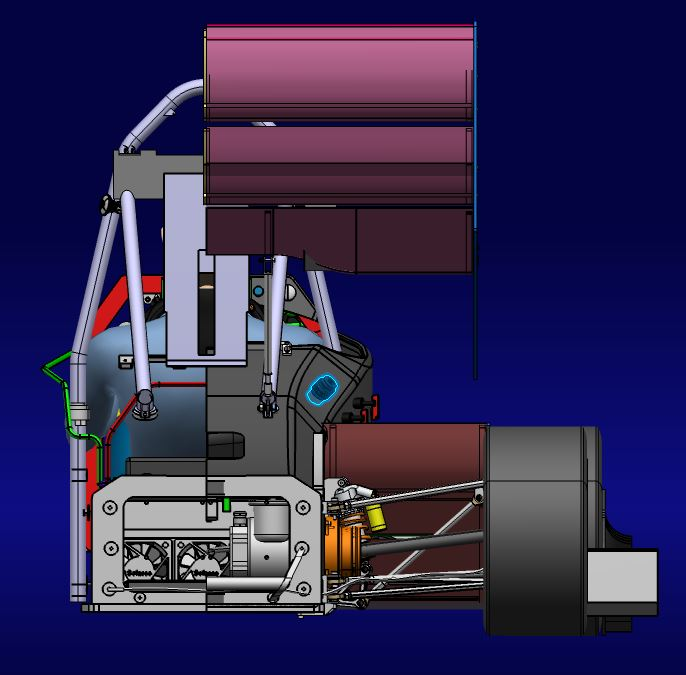
\includegraphics[width=\textwidth]{./img/hvd2.jpg}
	\caption{HVD envelope.}
	\label{fig:hvd2}
\end{figure}

\subsection{Ready-To-Drive-Sound (RTDS)}\label{subsec:RTDS}
%Responsible: Jano
% obrazky, schemata, rendery
% Dodelat odkazy a obrazky

\subsubsection{Description}
%Describe your concept of the RTDS, how the sound is produced, what are the parameters for activating the RTDS, etc.

We use piezo siren AE20M. The siren makes sound when \gls{ecub} recognize ready-to-drive state of car, it receives message from \gls{ecuf} about TS ON button while brake pedal is active (i.e. brake circuit is pressurised and the pressure information is reported by CAN message from \gls{ecup}) and \gls{sdc} is in non-error state. If message would be lost \gls{ecub} does not send confirmation status and \gls{ecuf} does not allow to activate ready to drive status. Sound pressure level of this siren is more than 90 dB(A) at 1 m, Output frequency is from 2.9 kHz. Controlling of \gls{rtds} is done by \gls{ecub} by transistor. \gls{rtds} beeps 2 seconds.

\begin{figure}[H]
	\centering
	\includegraphics[width=.5\textwidth]{./img/RTDS.pdf}
	\caption{\gls{ecub}.}
	\label{fig:RTDS}
\end{figure}

\subsubsection{Wiring, cables, current calculations, connectors}
%Describe wiring, show schematics, describe connectors and cables and show useful data regarding the wiring.

There are only two wires from \gls{ecub} to \gls{rtds} piezo siren, one switched by transistor and and the second is ground (block connections is on \ref{fig:RTDS-wiring}).

\begin{figure}[H]
	\centering
	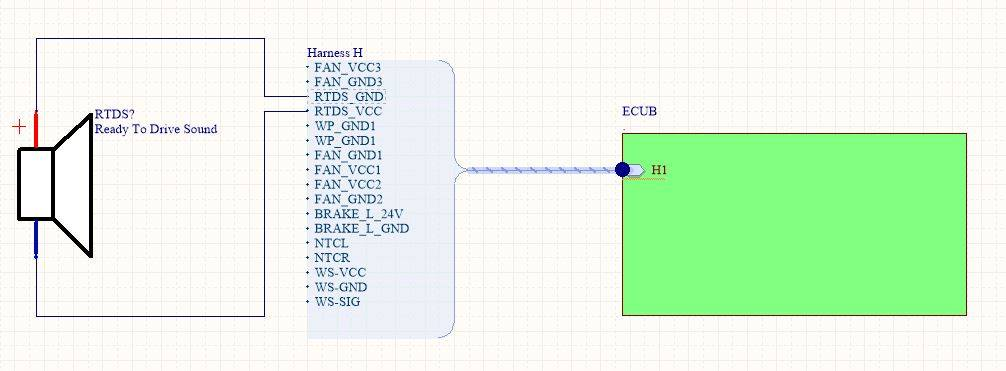
\includegraphics[width=\textwidth]{./img/rtds-wiring.jpg}
	\caption{RTDS wiring.}
	\label{fig:RTDS-wiring}
\end{figure}
\subsubsection{Position in car}
%Provide CAD-renderings showing all relevant parts. Mark the parts in the rendering, if necessary.

Ready to drive sound is placed on the top of \gls{acp} next to the \gls{mcr}, see \ref{fig:RTDS-position}.
\begin{figure}[H]
	\centering
	\includegraphics[width=\textwidth]{./img/rtds-position.jpg}
	\caption{\Gls{rtds} position.}
	\label{fig:RTDS-position}
\end{figure}

\newpage
\section{Accumulator}\label{sec:Accumualtor}
\subsection{HV Accumulator pack}\label{subsec:AccumulatorPack1}
%Responsible: Adam, JM
\subsubsection{Overview / description/parameters}
%Describe concept of accumulator pack, provide table with main parameters like number of cells, cell stacks separated by maintenance plugs, cell configuration, resulting voltages->minimum, maximum, nominal, currents, capacity etc.
Our accumulator pack is designed using 18650 Li-ion cells in 6 stacks configuration, active cooled by air. The accumulator pack contains cells, \gls{ams} modules (slaves), \gls{acp} main control unit (AMS master) with DC/DC converter, IMD unit, cooling fans and current sensor. There is smaller insulated box inside the accumulator pack, that accomodates \glspl{air} and main fuse.
Details are filled in following table:

\begin{table}[H]
	\centering
	\caption{Main accumulator parameters}
	\begin{tabularx}{\textwidth}{|X|X|}
		\hline
		Maximum Voltage: & 400 $V_{DC}$ \\[\TableSize]
		\hline
		Nominal Voltage: & 345.6 $V_{DC}$ \\[\TableSize]
		\hline
		Minimum Voltage: & 182 $V_{DC}$ \\[\TableSize]
		\hline
		Maximum output current: & 315 A (until any cell reaches 80 $^\circ$C) \\[\TableSize]
		\hline
		Maximum nominal current: & 270 A \\[\TableSize]
		\hline
		Maximum charging current: & 54 A \\[\TableSize]
		\hline
		Total numbers of cells: & 864 \\[\TableSize]
		\hline
		Cell configuration: & 96s9p \\[\TableSize]
		\hline
		Total Capacity: & 27.99 MJ \\[\TableSize]
		\hline
		Number of cell stacks < 120 $V_{DC}$ & 6 \\[\TableSize]
		\hline
	\end{tabularx}%
	\label{tab:acc-main}%
\end{table}%

\subsubsection{Cell description}
%Describe the cell type used and the chemistry, provide table with main parameters.

The used cell is the 18650 type cylindrical Li-ion cell. Detailed specification is shown in table below. Each cell has a \gls{cid} which disconnect the cell from others in parallel in case of cell failure (such an internal short circuit or over pressure) or in case of excessive discharge current. 

\begin{table}[H]
	\centering
	\caption{Main cell specification}
	\begin{tabularx}{\textwidth}{|X|X|}
		\hline
		Cell Manufacturer and Type & SONY VTC5A \\[\TableSize]
		\hline
		Cell nominal capacity: & 2.5 Ah \\[\TableSize]
		\hline
		Maximum Voltage: & 4.25 V \\[\TableSize]
		\hline
		Nominal Voltage: & 3.6 V \\[\TableSize]
		\hline
		Minimum Voltage:  & 2 V \\[\TableSize]
		\hline
		Maximum output current: & 35 A (until cell reaches 80 $^\circ$C) (14C)\\[\TableSize]
		\hline
		Maximum nominal output current: & 30 A(12C) \\[\TableSize]
		\hline
		Maximum charging current: & 6 A(2.4C) \\[\TableSize]
		\hline
		Maximum Cell Temperature (discharging) & 80 $^\circ$C \\[\TableSize]
		\hline
		Maximum Cell Temperature (charging) & 60 $^\circ$C \\[\TableSize]
		\hline
		Cell chemistry: & Lithium-Ion \\[\TableSize]
		\hline
	\end{tabularx}%
	\label{tab:acc-cell}%
\end{table}%

\subsubsection{Cell configuration}
%Describe cell configuration, cell interconnect, show schematics of electrical configuration and CAD of connection techniques, cover additional parts like internal cell fuses etc.

Cell configuration is 96s9p. Cells are divided into 6 stacks, configuration of each stack is 16s9p. Cells are connected by welding. Main cells interconnection is done by nickel sheet. This sheet is welded to each cell. There is additional copper sheet welded over the nickel sheet (for lowering resistance of the main current path).

 
\subsubsection{Cell temperature monitoring}
%Describe how the temperature of the cells is monitored, where the temperature sensors are placed, how many cells are monitored, etc. Show schematics, cover additional parts, etc.

	The cells’ temperature is monitored by \gls{ntc} temperature sensors. The manufacturer is TDK, type is: B57330V2103F260. Insulation of the sensors is done by 3M\textsuperscript{TM} PTFE Film Electrical Tape. Breakdown voltage of this tape 9.5 kV, operating temperature is 180 $^\circ$C. Thickness of this tape is 0.1 mm. Sensors are soldered in \glspl{pcb} that are covered with insulating tape and then mounted to each stack. 

\begin{figure}[H]
	\centering
	\includegraphics[width=\textwidth]{./img/ACP-stack.png}
	\caption{Stack configuration.}
	\label{fig:acp-stack}
\end{figure}

Position of temperature sensors on the top of each stack (highlighted objects)
\begin{figure}[H]
	\centering
	\includegraphics[width=\textwidth,trim={0cm 16cm 0cm 0cm}, clip]{./img/BMS-top-sensors.pdf}
	\caption{Top position of sensors.}
	\label{fig:bms-top}
\end{figure}
Position of temperature sensors on the bottom of each stack (highlighted objects)
\begin{figure}[H]
	\centering
	\includegraphics[width=\textwidth,trim={0cm 16cm 0cm 0cm}, clip]{./img/BMS-bottom-sensors.pdf}
	\caption{Bottom position of sensors.}
	\label{fig:bms-bottom}
\end{figure}
Top and bottom view of one stack 
\begin{figure}[H]
	\centering
	\includegraphics[width=\textwidth]{./img/BMS-top-andbottom.pdf}
	\caption{Rear and bottom view.}
	\label{fig:bms-top-and-bottom}
\end{figure}

\begin{table}[H]
	\centering
	\caption{General cell temperature parameters.}
	\begin{tabularx}{\textwidth}{|X|X|}
		\hline
		Temperature sensor accuracy: & 1\% \\[\TableSize]
		\hline
		Total number of cells: & 864 \\[\TableSize]
		\hline
		Total number of sensors: &  384 \\[\TableSize]
		\hline
		Max. distance from monitored negative cell terminal: & 2 mm \\[\TableSize]
		\hline
		\gls{ams} opens \glspl{air} during dis-charging if cell temperature is above: & 60 $^\circ$C \\[\TableSize]
		\hline
		\gls{ams} opens \glspl{air} during charging if cell temperature is above: & 60 $^\circ$C \\[\TableSize]
		\hline
	\end{tabularx}%
	\label{tab:acc-temp}%
\end{table}%

\subsubsection{Accumulator Management System}
%Describe the \gls{ams} used including at least the following:

\todo[inline]{Sem by to jeste chtelo neco napsat o pouzitem svabu.}

\begin{table}[H]
	\centering
	\caption{Cell voltage limits.}
	\begin{tabularx}{\textwidth}{|X|X|}
		\hline
		Minimum cell voltage (shutdown limit): & 2.2 V \\[\TableSize]
		\hline
		Maximum cell voltage (shutdown limit): & 4.2 V \\[\TableSize]
		\hline
		Measurement precision (mV): & $\pm$ 0.75 \\[\TableSize]
		\hline
	\end{tabularx}%
	\label{tab:acc-limits}%
\end{table}%

%\item Sense wiring protection (fusing / fusible link wire used)
%\item What upper and lower voltage does the AMS react at and how does it react?
%\item What cell temperature does the AMS react at and how does it react?
%\item Show tables of operation parameters
%\item Describe how many cells are sensed by each AMS board, the configuration of the cells, the configuration of the boards and how any communications wiring between boards is protected 
%\item Describe how the AMS is able to open the AIRs if any error is detected
%\item Describe where galvanic isolation occurs between TS and GLV system connections.

Each sense connection is protected with fuse. There are two types of fuses used: 

\noindent Littelfuse 0251001.MXL (Those are used, where the cells are contacted via \gls{pcb})

\noindent Eaton TR/3216LV1-R (Those are used, where measure wires are connected directly to cells)

Cell highest allowed voltage is 4.25 V so \gls{ams} reacts when the voltage is above 4.2 V. Cell lowest allowed voltage is 2 V so \gls{ams} reacts when the voltage is below 2.2 V. Reaching any of limits causes \glspl{air} disconnection.

Highest allowed temperature (by datasheet) for discharging is 80 $^\circ$C and for charging 60 $^\circ$C. Due to FSE rules our battery pack is limited to 60 $^\circ$C. \gls{ams} reacts when the temperature is higher than 60 $^\circ$C reaching limit causes \glspl{air} disconnection.

\paragraph{Recommended Operating Conditions}
TA = 25 $^\circ$C and TOP = 57.6 V; Min/Max values stated where TA = -40 $^\circ$C to 105 $^\circ$C and TOP = 12 V to 79.2 V (unless otherwise noted)
\begin{figure}[H]
	\centering
	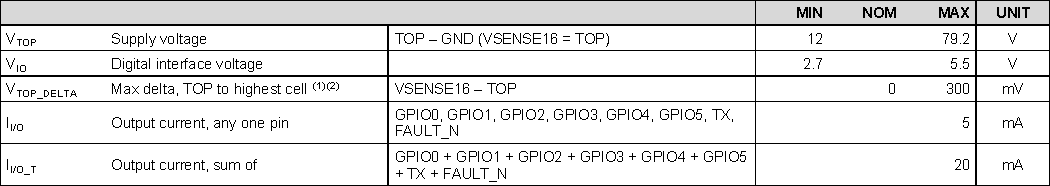
\includegraphics[width=\textwidth]{./img/BMS-operatingparms.pdf}
	\caption{Recommended operating parameters.}
	\label{fig:BMS-op-params}
\end{figure}


Each \gls{ams} board senses whole stack, that means it senses 144 cells, connected in 16s9p configuration. Communications wirings are protected by two 1kV 1nF capacitors CC1206KKX7RCBB102 by Yageo. There is placed one on each side (there is one on every \gls{ams}). The \gls{ams} is connected to Accumulator \gls{ecu} that has capability of direct \glspl{air} shutdown. The galvanic isolation between \gls{ts} and \gls{glvs} is done by two 1kV 1nF capacitors CC1206KKX7RCBB102 by Yageo. It is located on separated board connected between first \gls{ams} and Accumulator \gls{ecu}.




\subsubsection{Accumulator indicator}
%Describe the indicator, show wiring, provide tables with operation, PCB design, etc

We use LED indicator placed on Accumulator pack chassis. The LED is powered by a separate circuit which is also used to power the \gls{tsal}. The circuit function explanation is shared with \gls{tsal} HV part. 

\subsubsection{Wiring, cables, current calculations, connectors}
%Describe the internal wiring, show schematics, provide calculations for currents and voltages and show data regarding the cables and connectors used.
%	\item 	Discuss maximum expected current, DC and AC how long will this be provided?
%	\item Compare the maximum values to nominal currents
%	\item Give a table for each kind of wire in your tractive-system:
%	\item Describe your maintenance plugs, provide pictures
%	\item Use tables like the one shown below:


We use OLFLEX HEAT 180 SiF (see. \ref{app:PowerConductor})as Tractive System wires. Total gauge is 16mm2. Total ampacity is 165 A for main DC power buses. All other LV wiring in Accumulator is also done using OLFLEX HEAT 180 SiF wires with gauges ranging from 0,25 mm$^2$ to 1 mm$^2$. Basic data are given in tables below. We use 2 pin Deutsch ASHD connectors as HV Tractive system connectors as the Accumulator Pack outlet, Service box inlet and Motor controllers inlet. For Motor controllers outlets to motors we use 4 pin Deutsch ASHD connectors. Pins are rated each to 200 A of continuous current. According to our data from last season, average continuous DC current is expected to be to 80 A. The maximum DC current is to be 250 A for max. 5 seconds.

To ensure that connectors will withstand in-rush currents, we did following calculation. The most stressed connector is Accumulator pack outlet. The maximum power Motor Controllers will take is 80kW, which is 250A in maximum (depends on state of charge of accumulators). Based on heating a thermal capacity of mass of pins and nearest wiring, by power losses on contact resistance and temperature difference 50 $^\circ$C, these connectors will definitely withstand this current for more than 10 seconds, which is far ahead of motors overload capacity (cca. 4-5 seconds). Therefore, these connectors will never get to critical overload condition.


% Table generated by Excel2LaTeX from sheet 'List1'
\begin{table}[htbp]
	\centering
	\caption{Wire data of company A, 0.205 mm$^2$.}
	\begin{tabularx}{\textwidth}{|X|X|}\hline
		Wire type & OLFLEX HEAT 180 SiF \\[\TableSize]\hline
		Continuous current rating: & 165 A \\[\TableSize]\hline
		Cross-sectional area & $16mm^2$ \\[\TableSize]\hline
		Maximum operating voltage: &  500 V$_DC$\\[\TableSize]\hline
		Temperature rating: &  125 $^\circ$C\\[\TableSize]\hline
		Wire connects the following components: & Stacks $\,\to\,$ \glspl{air}, fuse $\,\to\,$ \gls{hv} Connector \\[\TableSize]\hline
	\end{tabularx}%
	\label{tab:acc-wire}%
\end{table}%

\begin{figure}[H]
	\centering
	\includegraphics[width=\textwidth]{./img/ACP-nut.png}
	\caption{Maintenance plugs I.}
	\label{fig:acp-maintance-plug}
\end{figure}

\begin{figure}[H]
	\centering
	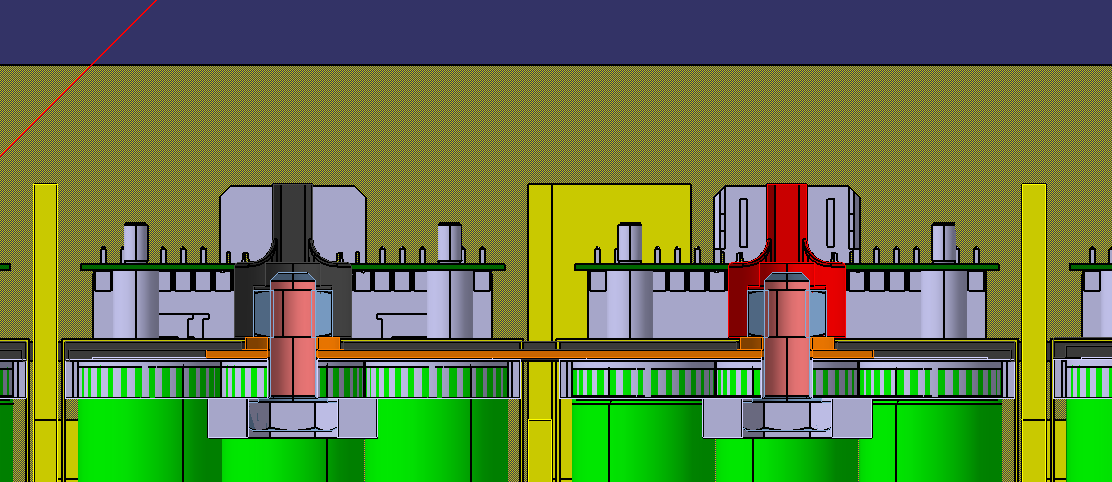
\includegraphics[width=\textwidth]{./img/ACP-nut2.png}
	\caption{Maintenance plugs II.}
	\label{fig:acp-maintance-plug2}
\end{figure}

\begin{figure}[H]
	\centering
	\includegraphics[width=\textwidth]{./img/ACP-view.png}
	\caption{Accumulator pack \gls{hv} wiring I.}
	\label{fig:acp-hv-wiring}
\end{figure}

\begin{figure}[H]
	\centering
	\includegraphics[width=\textwidth]{./img/ACP-fuse.png}
	\caption{Accumulator pack \gls{hv} wiring II.}
	\label{fig:acp-hv-wiring2}
\end{figure}

\subsubsection{Accumulator insulation relays}\label{subsubsection:airs}
%Describe the AIRs used and their main operation parameters, use tables, etc.

We use Kilovac EV200 as \glspl{air}, it is widely used standard contactor designed for EVs, working with inert gas atmosphere. Detailed specification is given in the following table:

% Table generated by Excel2LaTeX from sheet 'List1'
\begin{table}[H]
	\centering
	\caption{Basic AIR data.}
	\begin{tabularx}{\textwidth}{|X|X|}
		\hline
		Relay Type: & Kilovac EV200 \\[\TableSize]
		\hline
		Contact arrangement: & SPST \\[\TableSize]
		\hline
		Continuous DC current rating: & 500 A \\[\TableSize]
		\hline
		Overload DC current rating:  & 2000 A for 1 second \\[\TableSize]
		\hline
		Maximum operation voltage: & 900 V$_{DC}$ \\[\TableSize]
		\hline
		Nominal coil voltage: & 24 V$_{DC}$ \\[\TableSize]
		\hline
		Normal Load switching: & Make and break up to 650 A \\[\TableSize]
		\hline
		Maximum Load switching & 3 times at 2000 A \\[\TableSize]
		\hline
	\end{tabularx}%
	\label{tab:acc-air}%
\end{table}%

\subsubsection{Fusing}
%Describe the fuses used and their main operation parameters, use tables, etc.
%Additionally, fill out the following table for each fuse type used:

We use OEZ Varius P51T06 as the main fuse. It is intended to protect semiconductors. Both contactors and main fuse are enclosed in separate enclosure as it can be seen in the pictures above. Detailed specification is given in the following table:

\begin{table}[H]
	\centering
	\caption{Basic fuse data}
	\begin{tabularx}{\textwidth}{|X|X|}
		\hline
		Fuse manufacturer and type: & OEZ Varius P51T06 160A aR \\[\TableSize]
		\hline
		Continuous current rating:  & 160 A \\[\TableSize]
		\hline
		Maximum operating voltage  & 440 V$_{DC}$ \\[\TableSize]
		\hline
		Type of fuse: & High speed for semiconductors \\[\TableSize]
		\hline
		I2t rating: & 3300 A$^{2}$s \\[\TableSize]
		\hline
		Interrupt Current (maximum current at which the fuse can interrupt the current) & 50 kA \\[\TableSize]
		\hline
	\end{tabularx}%
	\label{tab:acc-fuse}%
\end{table}%

%Create a table with components and wires protected by the fuse(s) and the according continuous current rating, below is an example table with some potential entries.  Complete this table with information for your design and add/remove additional locations as applicable.  Ensure that the rating of all the components is greater than the rating of the fuse such that none of the other components become the fuse.

\todo[inline]{Tohle je ještě potřeba vyplnit!}

% Table generated by Excel2LaTeX from sheet 'List1'
\begin{table}[H]
	\centering
	\caption{Fuse Protection Table}
	\begin{tabularx}{\textwidth}{|X|X|X|X|X|}
		\hline
		Location & Wire Size & Wire Ampacity & Fuse type & Fuse rating\\[\TableSize]
		\hline
		Cells to AIRs & 6 AWG & 165 A & High-speed & 160 A \\[\TableSize]
		\hline
		AIR to Motor controller & 6 AWG & 165 A & High-speed & 160 A \\[\TableSize]
		\hline
		AIR to TSAL & 22 AWG & 5 A & High-speed & 3 A \\[\TableSize]
		\hline
		Accumulator output connector & 6 AWG & 165 A & High-speed  & 160 A \\[\TableSize]
		\hline
		Cells to AMS & N/A (PCB trace) & 5 A    & SMD    & 2 A \\[\TableSize]
		\hline
	\end{tabularx}%
	\label{tab:acc-fuse-protection}%
\end{table}%

\subsubsection{Charging}
%Describe how the accumulator will be charged. How will the charger be connected? How will the accumulator be supervised during charging? Show schematics, CAD-Renderings, etc., if needed
%Additionally, fill out the table:
We use self developed charger to charge our accumulator pack. Topologically it consist of galvanically isolated step-up transformer, followed by step-down "chopper" converter.
Charger is connected to the accumulator pack by separate low voltage and high voltage connector. They use \gls{can} bus to communicate, which goes through low voltage cord.
Charger is equipped with properly designed Shutdown Circuit, safety features...
\todo[inline]{Describe how the accumulator will be charged. How will the charger be connected? How will the accumulator be supervised during charging? Show schematics, CAD-Renderings, etc., if needed}
\todo[inline]{Honzo dopis to tady co vsechno umi a jak probiha proces rizeni nabijeni podle zakomentovaného zadani vyse.}

\begin{table}[H]
	\centering
	\caption{General charger data}
	\begin{tabularx}{\textwidth}{|X|X|}
		\hline
		Charger Type: & Self developed charger \\[\TableSize]
		\hline
		Maximum charging power: & 9 kVA  \\[\TableSize]
		\hline
		Maximum charging voltage: & 600 V \\[\TableSize]
		\hline
		Maximum charging current: & 25 A \\[\TableSize]
		\hline
		Interface with accumulator & CAN bus \\[\TableSize]
		\hline
		Input voltage: & 3x400 V, 50 Hz \\[\TableSize]
		\hline
		Input current: & 3x16 A \\[\TableSize]
		\hline
	\end{tabularx}%
	\label{tab:acc-charger}%
\end{table}%

\subsubsection{Mechanical Configuration/materials}
%Describe the concept of the container, show how the cells are mounted, use CAD-Renderings, show data regarding materials used, etc.

The whole mechanical structure of the case is made from sandwich structure, kevlar fiber and core, designed to be alternative structure. Basically the case is divided to main box, which is outer walls and floor, five longitudinal walls and one transverse wall divided this space on chambers for six stacks and space in front is used for additional technology (\gls{ecu}, \gls{imd}, \glspl{air}, Fuse, Current sensors, connectors etc.). AIR-Box is constructed of FR4 walls. The last component is lid, which is also the stacks holder, you can see in the picture.

Detailed stack composition is shown below in \ref{fig:acp-mech}. Cells are built in a support structure on each side and middle one. There are connecting plates made from welder of Ni201 alloy plate and copper CU99,99\% plate and spot-welded to respective cells. The entire stack is covered with an kevlar case. Each pole of a stack is ended by a copper terminal on the top of the stack. There are also vents hole at the cover and rear outer wall at main wall and also on both sides of stack, cells are cooled by air flowing among them. \gls{bms} board is placed on the top of each stack.

\begin{figure}[H]
	\centering
	\includegraphics[width=\textwidth]{./img/acp-mech.png}
	\caption{Mechanical fastening of \gls{acp}.}
	\label{fig:acp-mech}
\end{figure}

\subsubsection{Position in car}
%Provide CAD-renderings showing the relevant parts. Mark the parts in the rendering, if necessary.  Ensure that the required mechanical structure to protect the accumulator and other electrical components is clearly identified.

\begin{figure}[H]
	\centering
	\includegraphics[width=\textwidth]{./img/acp-position.jpg}
	\caption{Position of \gls{acp} in car.}
	\label{fig:ACP-position}
\end{figure}



\subsection{GLVS Accmulator}
\subsubsection{Description}
Our \gls{glvs} Accumulator is made using 18650 Li-ion cells Sony VTC-5. The configuration is 6s1p which equals to our low-voltage system voltage 24 V. Datasheet is in appendix.

\subsubsection{Battery management}

An LTC6084 chip is used to monitor individual cells in the LV battery. The circuit and software are part of ECU-B, which is the unit which also controls power to the rest of GLVS.

Undervoltage condition is checked continuously during vehicle operation; if the voltage of any cell falls below the specified range for several measurements in a row, the battery is cut off. If the HV-to-LV DCDC Converter was able to start in time, it will continue to power GLVS. Otherwise GLVS will shut down.

Overvoltage condition is monitored only when the LV battery is being charged. The cut-off for each cell is slightly below the specified maximum, to account for measurement uncertainty and to extend cell life.

\subsubsection{Wiring, cables, current calculations, connectors}
%Describe wiring, show schematics, describe connectors and cables and show useful data regarding the wiring.  Include information on the working voltage and current rating of the accumulator.

The \gls{glvs} Accumulator is made of 18650 cells. They are held together by modular structure and interconnected by nickel tabs using spot welding. On each end, there is small tab spot welded to the cell and main wire soldered on the tab. On the other end of the mains wire (positive and negative), there is a XT-60 connector soldered. Balancing wires are soldered to the respective interconnecting tabs. The battery use 7-pin balancing connector JST-XH, so that the whole accumulator is using standards widely used in RC models. The intent is to have the ability to use wide range of diagnostic tool or chargers made to this standard.

The battery also have 4 \glspl{ntc} for measuring cells temperature connected by separate connector.

The peak discharge rating of the cells is 30 A, the XT-60 connector continuous current rating is 60A. The corresponding input in \gls{ecub} where the accumulator is connected is fused by 20 A main fuse. The wire used for mains between the cells and XT-60 connector is silicone insulated copper cable of cross-section 2.5 mm$^2$ which gives ampacity of 30 A, well above the fuse.

The balancing wires are AWG22 with ampacity 5 A and each is fused with 2 A SMD fuse at the \gls{pcb} behind the JST-XH connector.

\begin{table}[H]
	\centering
	\caption{GLVS accumualtor general parameters.}
	\begin{tabu}{|X|X|}\hline
		Cell/Accumulator: & Sony VTC-5 18650 Li-ion\\\hline
		Accumulator configuration – parallel: & 1 \\\hline
		Accumulator configuration – series: & 6 \\\hline
		Maximum Voltage: & 25.2 V \\\hline
		Nominal Voltage: & 21.6 V \\\hline
		Minimum Voltage: & 12 V \\\hline
		Max. Continuous Discharge Current: & 20 A \\\hline
		Peak Discharge Current: & 30 A \\\hline
		Peak Discharge Current Time: & Till temp rise to 80 \degC (refer to \hyperref[app:sony-vtc5]{datasheet}, section 2.8.2) \\\hline
		Max. Continuous Charge Current & 4 A\\\hline
		Total capacity[MJ]: & 0.194 MJ \\\hline
	\end{tabu}%
	\label{tab:LVbatt-general}%
\end{table}%

GLVS cell datasheet: \ref{app:sony-vtc5}

\subsubsection{Position in car}
Positon of whole ECUB can be seen here \ref{fig:ecub_position}.
\begin{figure}[H]
	\centering
	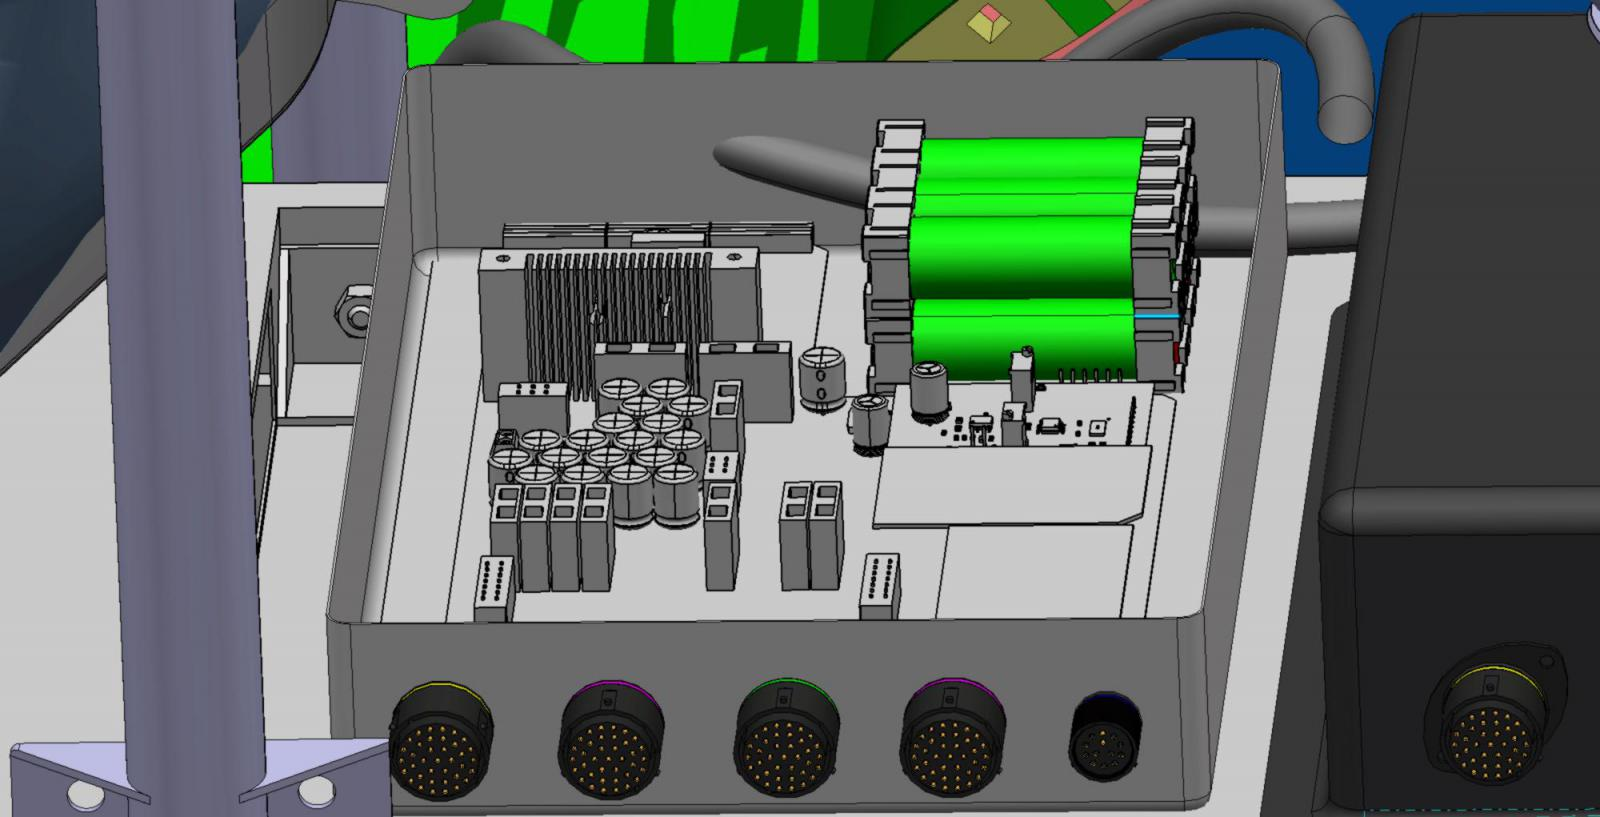
\includegraphics[width=\textwidth,clip]{./img/ECUB_BATTERY_POSITION.jpg}
	\caption{\gls{glvs} battery position.}
	\label{fig:GLVS_battery_position}
\end{figure}


\newpage
\section{Energy meter mounting}\label{sec:DataLogger}
%Responsible: Kosina
\subsection{Description}
%Describe where the energy meter is mounted and how, etc.

The energy meter is mounted in Service Box, which also contains power cable terminals and BSPD. Energy meter will have dedicated space in Service box with stoppers preventing it from moving. 

\subsection{Wiring, cables, current calculations, connectors}
%Describe the wiring, show schematics, provide calculations for currents and voltages, and show data regarding the cables and connectors used.

The energy meter is powered from ECUB (part of Harness\_G) with connector G1 to Service box. Voltage measuring is done by connecting Energy meter to power cable terminals, which are also in Service box. This is done by Olflex Heat 180 SiF wires rated for 500V and size AWG 17. Having power terminals in Service box allow us to measure current using current probe, or by connecting Energy meter directly to Tractive system path(both poles are possible). This is also done by Olflex Heat 180 SiF wires, but with cross-sectional area of 16mm2 and rated for 500V and 165A. For power cable datasheet see \ref{app:PowerConductor}

\subsection{Position in car}
%Provide CAD-renderings showing all relevant parts. Mark the parts in the rendering, if necessary.

Energy meter is placed in box we call “Service Box”. The box is carbon fiber lined with FR-4 from inside. Position in car is shown below in \ref{fig:ServiceBox-position}.

\begin{figure}[H]
	\centering
	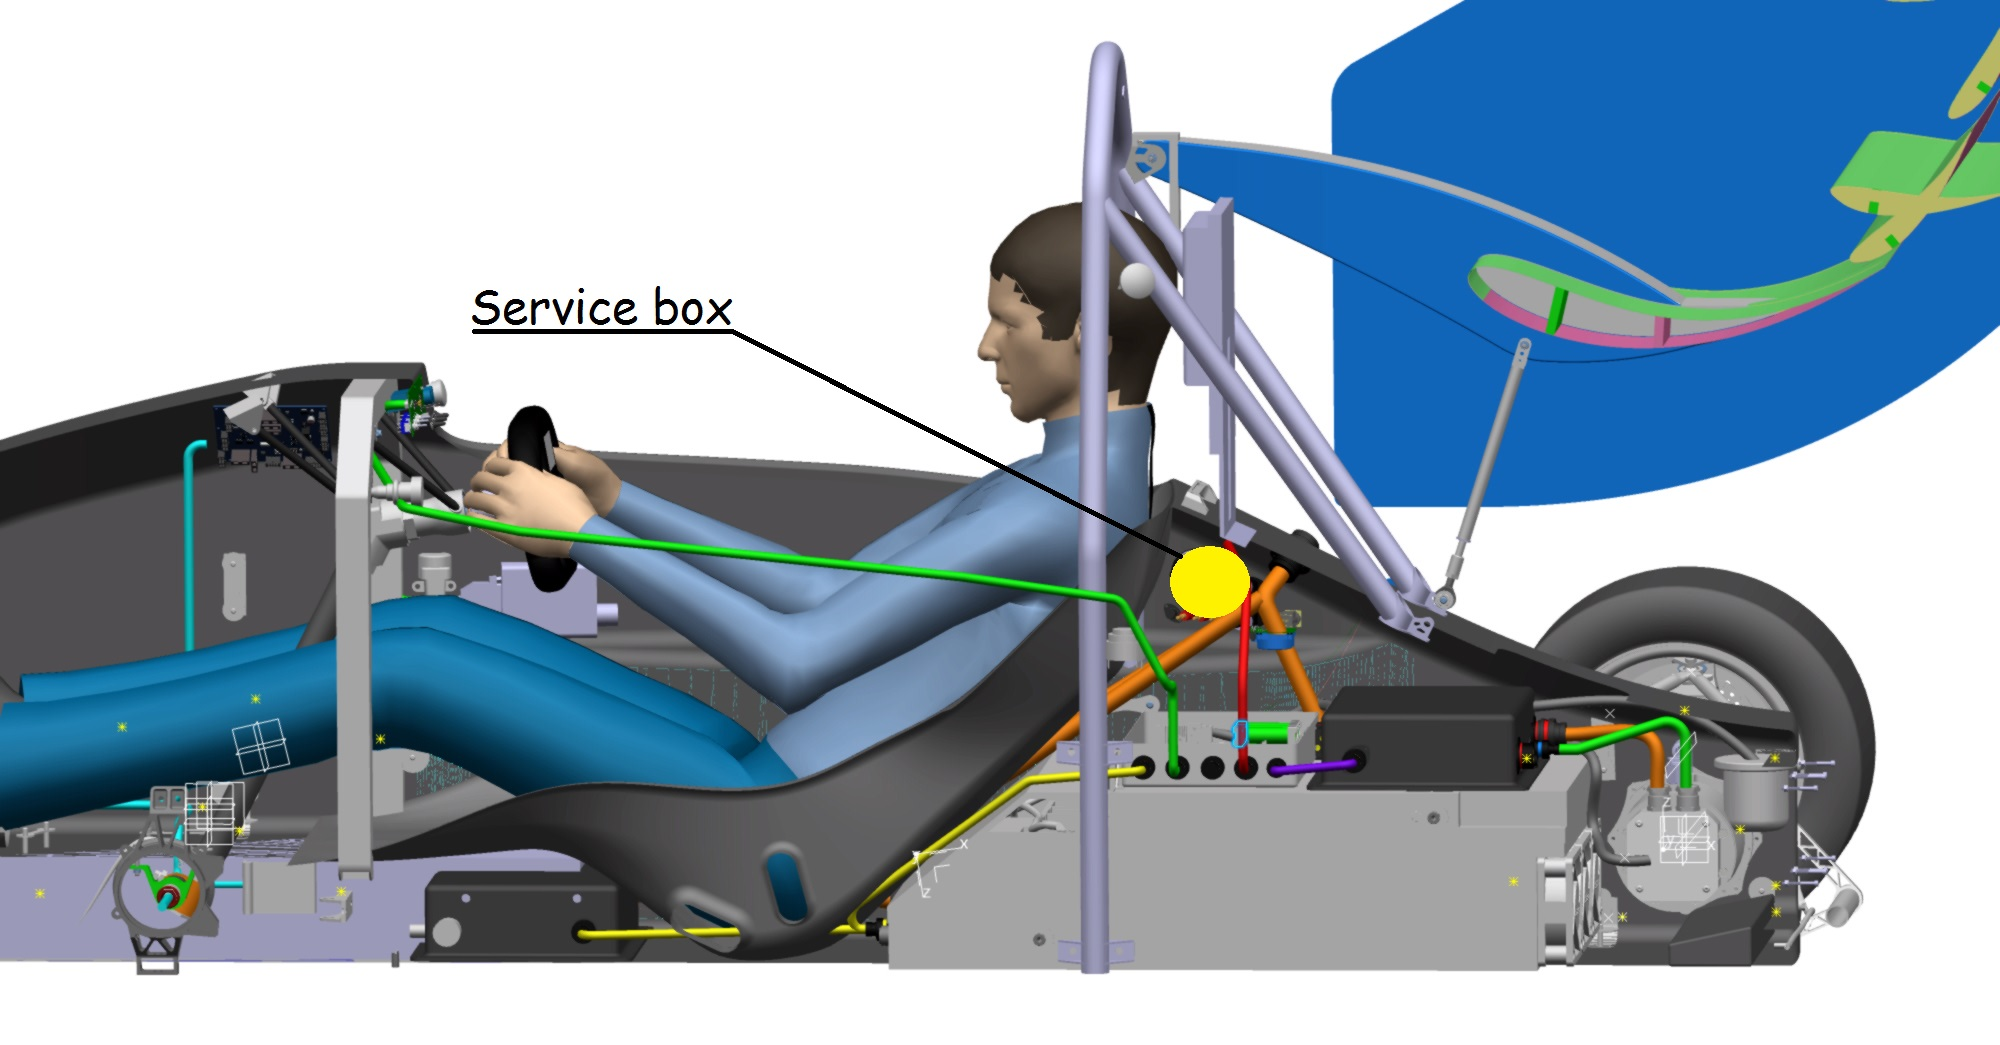
\includegraphics[width=\textwidth]{./img/ServiceBox-position.jpg}
	\caption{Service box position.}
	\label{fig:ServiceBox-position}
\end{figure}







\newpage
\section{Motor Controller}\label{sec:MotorController}
%Res:Hotovo
%Kontrola kabelaze
\subsection{Motor Controller 1}
% Kabeláž
% add schematic and datasheet

\subsubsection{Description, type, operation parameters}
%Describe important functions; provide table with main parameters like resulting voltages->minimum, maximum, nominal, currents etc.
Motor controller is a prototype of MiRy X-Boss Motor Controller. It is fully self-designed for driving 2 \gls{pmsm} motors simultaneously with Resolver sensors as a position feedback. Field Oriented Control is implemented with galvanic isolated current sensors LEM HTFS 200-P.

Galvanic isolation on PCB is shown in \ref{app:mc-top} and \ref{app:mc-bot}. The only place where isolation is smaller then required 4mm is between pins of DC/DC NME1215SC. Real space gap is 1.54 mm. The NME1215SC has rated voltage of 1kV. See \ref{app:NME1215SC}.

Motor Controller communicate with traction control unit by private CAN bus. If any error occurs in their communication – Motor Controller stops driving both motors (error mode). It also implements discharge circuit which is activated by CAN or in case of Auxiliary supply disconnection (resistors are driven by normally-closed relay).

A current limit is set to not overload used motors. For each motor controller different. Rear motor controller has set peak current limit to 202 A and temperature limit to 120 $^\circ$C. Front Motor Controller’s current limit is 70 A and temperature limit also 120 $^\circ$C.

\begin{table}[H]
	\centering
	\caption{General motor controller data}
	\begin{tabularx}{\textwidth}{|X|X|}\hline
		Motor controller type: & MiRy X-Boss \\[\TableSize]\hline
		Maximum continuous power: & 2 x 90 kW (in:400 V, out:200 A) \\[\TableSize]\hline
		Maximum peak power: & 2 x 146 kW for 5s (in:400 V, out:300 A) \\[\TableSize]\hline
		Maximum Input voltage: & 410 V$_{DC}$ \\[\TableSize]\hline
		Output voltage: & 282 V$_{AC}$ \\[\TableSize]\hline
		Maximum continuous output current: & 2 x 200 A \\[\TableSize]\hline
		Maximum peak current: & 2 x 300 A for 5s \\[\TableSize]\hline
		Control method: & CAN \\[\TableSize]\hline
		Cooling method: & Water \\[\TableSize]\hline
		Auxiliary supply voltage: & 24 V$_{DC}$ \\[\TableSize]\hline
	\end{tabularx}%
	\label{tab:MC:general}%
\end{table}%

\subsubsection{Wiring, cables, current calculations, connectors}
%Describe the wiring, show schematics, provide calculations for currents and voltages and show data regarding the cables and connectors used.

Motor controllers are connected with HVD box by high voltage cable. High current connector “ASHD 0 22-24320 P N” by Deutsch is used. 

\begin{table}[H]
	\centering
	\caption{Wire data of OLFLEX HEAT 180}
	\begin{tabularx}{\textwidth}{|X|X|}\hline
		Wire type: & OLFLEX HEAT 180 SiF  \\[\TableSize]\hline
		Current rating: & 165 A \\[\TableSize]\hline
		Fuse current rating: & 160 A \\[\TableSize]\hline
		Maximum operating voltage: & 500 V \\[\TableSize]\hline
		Temperature rating: & 180 $^\circ$C \\[\TableSize]\hline
	\end{tabularx}%
	\label{tab:MC:wire}%
\end{table}%

%table
\subsubsection{Position in car}
%Provide CAD-renderings showing the relevant parts. Mark the parts in the rendering, if necessary.

The position of both motor controllers is shown in \ref{fig:MC:position}.

\begin{figure}[H]
	\centering
	\includegraphics[width=\textwidth]{./img/MC-position.jpg}
	\caption{MC position.}
	\label{fig:MC:position}
\end{figure}
\subsection{Motor Controller 2}
%If identical parts are used, just refer to the corresponding sections, don’t copy and paste.
Motor controller 2 is identical as Motor controller 1.






\newpage
\section{Motors}\label{sec:Motors}
%res: Nove datasheet
%Kontrola ale nakopirovano
\subsection{Motor 1}

\subsubsection{Description, type, operation parameters}
%Describe the motor used, provide table with main parameters like resulting voltages->minimum, maximum, nominal, currents, resulting motor power, use figures to show important characteristics.

We are using prototype motors from company TG Drives. They developed prototype motors with special parameters and water cooling. We are using two motors on rear axle (motor 1) and two motors on front axle.
\begin{table}[H]
	\centering
	\caption{General motor 1 data}
	\begin{tabu}{|X|X|}\hline
		Motor Manufacturer and Type: & TG Drives – N5-1600-100-380a-h-special-v2 \\\hline
		Motor principle & PMSM \\\hline
		Maximum continuous power: & 11.5 kW \\\hline
		Peak power: & 35 kW \\\hline
		Input voltage: & 260 V$_AC$ \\\hline
		Nominal current: & 38.2 A \\\hline
		Peak current: & 171 A \\\hline
		Maximum torque: & 48 Nm \\\hline
		Nominal torque: & 11 Nm \\\hline
		Cooling method: & Water \\\hline
	\end{tabu}%
	\label{tab:motors1-general}%
\end{table}%

\begin{figure}[H]
	\centering
	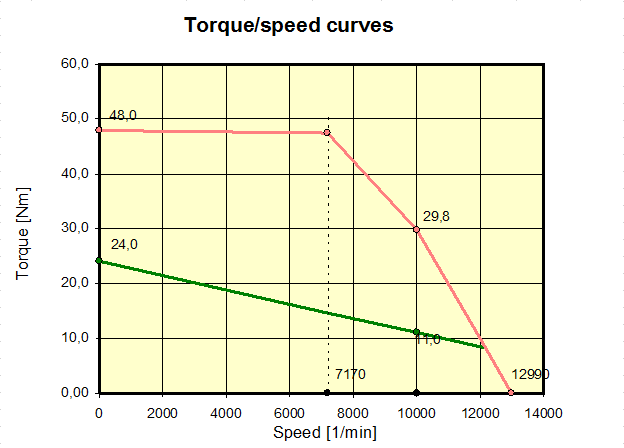
\includegraphics[width=\textwidth]{./img/MOTOR1-torque.png}
	\caption{Rear motor characteristics.}
	\label{fig:torque1}
\end{figure}

\iffalse\begin{itemize}
\item 	Give a plot of power vs. Rpm including a line for nominal and maximum power
\item give a plot of torque vs. rpm including a line for nominal and maximum torque
\end{itemize}\fi

\subsubsection{Wiring, cables, current calculations, connectors}
We use Raychem TR 16-10-0 and TR 16-6-0. There are leadthrough used for cables in motors and connectors Souriau „8STA 0 18 18” are used in Motor controllers.

\subsubsection{Position in car}
%Provide CAD-renderings showing all relevant parts. Mark the parts in the rendering, if necessary and clearly identify the structure used to protect all relevant parts.

Rear motors are situated in the rear-most part of the frame. 

\begin{figure}[H]
	\centering
	\includegraphics[width=\textwidth]{./img/Motor-rear-position.jpg}
	\caption{Rear motor position.}
	\label{fig:Motor-rear-position}
\end{figure}

\subsection{Motor 2}% Front

\begin{table}[H]
	\centering
	\caption{General motor 2 data}
	\begin{tabu}{|X|X|}\hline
		Motor Manufacturer and Type: & TG Drives – M4-0470-90-380a-h-special-water-cooling-lfe-60mm \\\hline
		Motor principle & PMSM \\\hline
		Maximum continuous power: & 4.2 kW \\\hline
		Peak power: & 8.2 kW \\\hline
		Input voltage: & 260 V$_AC$ \\\hline
		Nominal current: & 12.2 A \\\hline
		Peak current: & 67 A \\\hline
		Maximum torque: & 16.2 Nm \\\hline
		Nominal torque: & 4.4 Nm \\\hline
		Cooling method: & Water \\\hline
	\end{tabu}%
	\label{tab:motors2-general}%
\end{table}%

\begin{figure}[H]
	\centering
	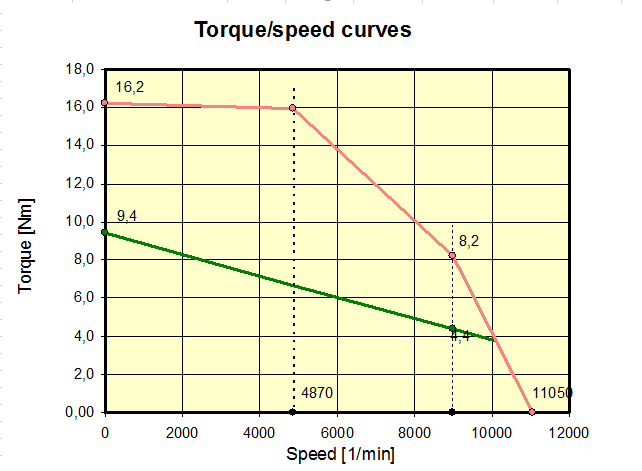
\includegraphics[width=\textwidth]{./img/MOTOR2-torque.png}
	\caption{Front motor characteristics.}
	\label{fig:torque2}
\end{figure}


\subsubsection{Wiring, cables, current calculations, connectors}
We use Raychem TR 16-10-0 and TR 16-6-0. There are leadthrough used for cables in motors and connectors Souriau „8STA 0 18 18” are used in Motor controllers.

\subsubsection{Position in car}
Front motors are situated directly in the front uprights.

\begin{figure}[H]
	\centering
	\includegraphics[width=\textwidth]{./img/Motor-front-position.jpg}
	\caption{Front motor position.}
	\label{fig:Motor-front-position}
\end{figure}




\newpage
\section{Torque Encoder}\label{sec:TorqueEncoder}
%Responsible: Bacha
%ECUP
\subsection{Description/additional circuitry}
Car is using two torque encoders for accelerator pedal. Encoders are linear potentiometers. Sensors are powered and measured by \gls{ecup}. They output analog voltage signal equal to accelerator pedal position. Both output signals goes through \ref{fig:ecup_analog_input} and low pass filters. Then they are fed to \gls{adc} and analyzed by \gls{mcu} for validity and plausibility. Information about position and errors is send though \gls{can}.

\begin{table}[H]
	\centering
	\caption{Torque encoder data}
	\begin{tabu}{|X|X|}
		\hline
		Torque encoder manufacturer: & TE connectivity  \\\hline
		Torque encoder type: & MLP-50  \\\hline
		Torque encoder principle: & linear potentiometer  \\\hline
		Total number of Torque Encoder Sensors: & 2  \\\hline
		Supply voltage: & +5 V  \\\hline
		Maximum supply current: & 1 mA  \\\hline
		Operating temperature: & -30 \degC to -150 \degC  \\\hline
		Used output: & DC voltage 0 V to 5 V\\\hline
	\end{tabu}%
	\label{tab:encoder-general}%
\end{table}%

Full datasheet: \ref{app:torque_encoder_datasheet}

\subsection{Torque Encoder Plausibility Check}
Torque encoder implausibility, short circuit and open circuit checks are done by \gls{mcu}. Sensors are powered from +5V. Used travel of sensors does not contain end positions. Converted analog signal ranges are normalized according to calibration.
If any following sensor error is detected, motor controllers are shut down and message is send through \gls{can} to other units.

\paragraph{Electrical check} 
Using only part of whole range of sensor excluding end positions allows detection of signal short to Ground or voltages higher or equal to sensor's power voltage.

Analog input circuitry of \gls{ecup} is shown in \ref{fig:ecup_analog_input}. In normal conditions, signal from sensor (RAW) goes through $R_2$, then is clamped by $D_1$ and continues through $R_1$ and $C_1$ to filters and other circuits of \gls{ecup} (AIN). TEST signal is held \textit{low} but due to high resistance of $R_3$ has minimal impact on input signal.

When \gls{adc} measures 0V or value close to 0V, TEST signal logic level is switched \textit{high} to charge $C_1$ through $R_3$. After short while, logic level of TEST signal is read back. If \textit{high} logic level is read, sensor input is evaluated as \textit{open circuit}, otherwise it is \textit{short circuit} to GND. If measured value is close to power voltage of sensor or above measurable range, it is evaluated as \textit{short circuit} to power voltage or higher.

\paragraph{Implausibility}
Position values difference is calculated and compared with maximal allowed error threshold (10\%).

\begin{figure}[H]
\begin{center}
	\includegraphics[width=0.5\textwidth]{./img/ECUP_AIN.pdf}
	\caption{\gls{ecup} analog input circuit}
	\label{fig:ecup_analog_input}
\end{center}
\end{figure}



\subsection{Wiring}
\ref{fig:ecup_wiring} is diagram of wiring between accelerator pedal sensors and \gls{ecup}.

\begin{figure}[H]
\begin{center}
	\includegraphics[width=0.5\textwidth]{./img/ECUP_wiring.pdf}
	\caption{ECU-P sensor wiring}
	\label{fig:ecup_wiring}
\end{center}
\end{figure}

\subsection{Position in car/mechanical fastening/mechanical connection}
In \ref{fig:torque_encoder_position} is shown position of two torque encoder sensors (piston shape objects).

\begin{figure}[H]
\begin{center}
	\includegraphics[width=\textwidth]{./img/ACC-pedal-pos.jpg}
	\caption{Torque encoder position}
	\label{fig:torque_encoder_position}
\end{center}
\end{figure}



%\begin{figure}[H]
%\begin{center}
%	\includegraphics[width=0.8\textwidth]{./img/ACC-pedal-pos2.jpg}
%	\caption{Torque encoder position}
%	\label{fig:torque_encoder_position_alt}
%\end{center}
%\end{figure}




\newpage
\section{Brake Encoder}\label{sec:BrakeEncoder}%added
%Responsible: Bacha
%ECUP
\subsection{Description/additional circuitry}
Car is using two pressure sensors as encoders for brake pedal. Each one is for separate brake system. Sensors are powered and measured by \gls{ecup}, same unit as \ref{sec:TorqueEncoder}. Pressure sensors output analog voltage signal equal to brake system pressure. 

%\def\tabularxcolumn#1{m{#1}}

\begin{table}[H]
	\centering
	\caption{Brake encoder data}
	\begin{tabularx}{\textwidth}{|X|X|}
		\hline
		Torque encoder manufacturer: &  Keller \\[\TableSize]\hline
		Torque encoder type: & PA-21 Y \\[\TableSize]\hline
		Torque encoder principle: & pressure sensor \\[\TableSize]\hline
		Total number of Torque Encoder Sensors: & 2 \\[\TableSize]\hline
		Supply voltage: & +24 V \\[\TableSize]\hline
		Maximum supply current: &  4 mA  \\[\TableSize]\hline
		Operating temperature: & -40 $^\circ$ to 100 $^\circ$C \\[\TableSize]\hline
		Used output: & DC voltage 0.5 V to 4.5 V \\[\TableSize]\hline
	\end{tabularx}%
	\label{tab:brake-general}%
\end{table}%

\begin{figure}[H]
	\begin{center}
		\includegraphics[width=\textwidth]{./img/BRK-pos.jpg}
		\caption{Pressure sensor positon.}
		\label{fig:brake_pressure_position}
	\end{center}
\end{figure}

\subsection{Brake Encoder Plausibility Check}
Implausibility is not checked, because eForce does not use brake pedal information to control \glspl{mc}.

%
%\subsection{Wiring}
%Describe the wiring, show schematics, show data regarding the cables and connectors used.
%
%\subsubsection{Position in car/mechanical fastening/mechanical connection}
%Provide CAD-renderings showing all relevant parts and discuss the mechanical connection of the sensors to the pedal assembly. Mark the parts in the rendering, if necessary.






\newpage
\section{Additional LV-parts interfering with tractive system}\label{sec:AdditionalLV}
\subsection{VDCU(Vehicle Dynamics Control Unit)}
It is \gls{ecu} that manipulates torque request from driver pedal to calculate final torque for all 4 motors. The calculated torque never exceed driver request as driver request is processed as torque limitation Traction control can only decrease the total amount of requested torque.

\subsubsection{Description}
Board uses only LV and 2x \gls{can} bus.

HW :
\begin{itemize}
	\item Texas Instruments C2000 Delfino F28377 \gls{mcu}
	\item 5 V can transceiver TJA1049
\end{itemize}

\noindent SW:\\
Board is programmed using simulink embedded coder. Advantage is that we can use our developed code for IPG Carmaker simulation (MIL) directly into our formula. \gls{vdcu} uses pedal position, inertial measurement, steering wheel sensor, wheel speed sensor and motor encoders to manipulate the torque. Measurements are fed into our yaw rate control system. Output is a torque vector fed to torque vectoring algorithm that calculates the torque distribution for all wheels The resultant torque for individual wheels is lowered by traction control algorithm if needed and fed to motors.

\begin{figure}[H]
	\centering
	\includegraphics[width=\textwidth]{./img/VDCU-pcb.jpg}
	\caption{\gls{pcb} of \gls{vdcu}.}
	\label{fig:VDCU-pcb}
\end{figure}

\subsubsection{Wiring, cables}
Module is connected using headers to \gls{ecub}.

\subsubsection{Position in car}
Inside \gls{ecub} box.

\subsection{LV part 2}
\todo[inline]{Describe those parts here which interfere or influence the tractive system, for example a controlling unit that measures wheel speeds and steering angle and calculates a target torque for each motor or a DC/DC-Converter providing power for the LV-system from the HV-system, etc.}
\todo[inline]{wheel speed - ECUB}
\todo[inline]{steering wh. angle - ECUP}

\subsection {DC/DC-Converters for the car GLVS and ACP cooling fans}\label{subsec:glvs_dcdc}
Two additional DC/DC converters are present in the \gls{acp}, within the \gls{ecua}. The first DC/DC supplies the car \gls{glvs} with 24 V. The second one is the power supply for \gls{acp} cooling fans. Both DC/DC converters are of the same type, CINCON, CFB600-300S24. This type converter is an isolated type, 3000 V$_{AC}$ min., as per the device datasheet. (\ref{app:glvs_dcdc}). The \gls{glvs} is therefore safely isolated from the \gls{hv}, same applies for the \gls{acp} cooling system, that is also isolated from the car \gls{glvs}, due to having a separate DC/DC converter. DC/DC inputs are fused by a FU$_1$, fast blow 2A 500V rated fuse (\ref{app:dcdc_fuse_datasheet}).

\subsubsection{Description}

\begin{figure}[H]
	\centering
	\includegraphics[width=\textwidth,clip]{./img/ECUA_DCDC_PRECHARGE.pdf}
	\caption{DC/DC pre-charge circuit and switching schematic.}
	\label{fig:precharge_dcdc_sch}
\end{figure}

Overall block diagram of the DC/DC circuitry is in \ref{fig:precharge_dcdc_sch}. Both DC/DC converters DCDC$_1$ and DCDC$_2$ share the same HV supply circuit, fused by fuse FU$_1$. Both DC/DC converters are isolated from the \gls{acp} \gls{hv} using relay RE$_1$. As additional DC link capacitors $C_{dclink}$ are required for the converters on the input HV side, a separate pre-charge circuit is also required. 
Relays type is Finder 40.52 (\ref{app:precharge_relay_datasheet}), two contacts always series connected to enhance the DC breaking capacity. Both DC/DC converters are always switched off first using their dedicated ON/OFF inputs, therefore there is no requirement for full DC current breaking capacity for the relays RE$_1$ and RE$_2$. In case of failure of one of the DC/DC converters, a fuse FU$_1$ will act to protect against further damage. 

\paragraph{Failure behavior and response}
\begin{itemize}
	\item Failure of the RE$_1$ relay in closed position only presents risk of draining the \gls{acp} charge away because of the pre-charge current and stand-by currents of both DC/DC converters. As the stand-by current of both DC/DC converters is negligible and the state of the HV circuitry of the DC/DC converters is monitored using the measurement circuitry block, the \gls{ecua} maintenance members can be notified of the failure, using the car diagnostics over the CAN bus. 
	
	\item RE$_1$ failing open presents no risk, as none of the DC/DC converters will work (\gls{acp} cooling failure, \gls{glvs} supply failure) and both the car would not be able to turn on properly and transition to the TS ON state.
	The measurement block of the DC/DC converter \gls{hv} input side is supplied using a small auxiliary isolated DC/DC converter (\ref{app:aux_dcdc_datasheet}). Signaling from the measurement block to the \gls{glvs} control side of the car is done utilizing a combination of digital signal isolator, SiLabs Si8600 series (\ref{app:ecua_isloator_datasheet}).
\end{itemize}


Both DC/DC converters DCDC$_1$ and DCDC$_2$ are fully protected against continuous overload or short circuit condition on their output, as specified in the device datasheet. Additional isolated current sense circuits are used on both converters, using a hall effect sensor, type ACS712 from Allegro \ref{app:acs712_datasheet}. These sensors are only informative, used only for diagnostic purposes to measure current consumption from the car's \gls{glvs} system and \gls{acp} cooling.

\subsubsection{Wiring, cables}
All wiring in \gls{acp} is described in \ref{subsec:acp_wiring}.

\subsubsection{Position in car}
The DC/DC converters and all their associated circuitry are present on the \gls{ecua} PCB. \gls{ecua} is located withing the \gls{acp} container, in a separated compartment neighbouring the AIR box. Please see \ref{fig:ECUA} for details about the \gls{acp} container component placement.


\subsection{LV part 2}
\todo[inline]{Describe those parts here which interfere or influence the tractive system, for example a controlling unit that measures wheel speeds and steering angle and calculates a target torque for each motor or a DC/DC-Converter providing power for the LV-system from the HV-system, etc.}
\todo[inline]{wheel speed - ECUB}
\todo[inline]{steering wh. angle - ECUP}


\newpage
\section{Overall Grounding Concept}\label{sec:GroundingConcept}
%Zalaminovat, kopie
\subsection{Description of the Grounding Concept}
Rear wing is not grounded, there is no \gls{ts} nor \gls{glvs} electronics within 100mm range.
Front and side wings are grounded with wires that are connected to their (metal) mounting screws and \gls{glvs} ground.
Steering wheel is grounded using wire connected to \gls{glvs} ground.

\subsection{Grounding Measurements}
To verify, that our grounding concept is compliant with rules, we are using 4 point resistance measurement method between parts and \gls{glvs} ground with current power supply to ensure resistance below 5 \ohm.


\newpage
\section{Firewall}\label{sec:Firewall}
%Responsible: hotov
\subsection{Description/materials}
%Describe the concept, layer structure and the materials used for the firewall. Show how the low resistance Control System ground connection is achieved.

We are using standard concept of firewall as described in the rules (T4.5.4). So the firewall is made from 2 layers. The first one is 0,5 mm thick aluminum sheet and the second one is 0,8 mm thick glass fiber/polyester plastic sheet with UL 94-V0 certificate (type: UPM 203 / UPM 71/S included in appendix). These are glued together and bended to the shape of final firewall. Aluminum sheet is oriented to the dangerous side and glass fiber to the driver side.

\subsubsection{Position in car}
%Provide CAD-renderings showing all relevant parts. Mark the parts in the rendering, if necessary.

Firewalls are located behind the seat and above the front motor controller (under drivers knees). These firewalls are connected with "firewall tunnel" where are located the high voltage cables.

\begin{figure}[H]
	\centering
	\includegraphics[width=\textwidth]{./img/Firewall-position.jpg}
	\caption{Firewall position.}
	\label{fig:Firewall-position}
\end{figure}

%------Appendix------
\appendix
%\setcounter{figure}{0} 
\renewcommand{\figurename}{Appendix}

\section{Appendix}\label{sec:Appendix}

\subsection{HV Disconnect (HVD)}

\begin{figure}[H]
	\centering
	\includegraphics[width=\textwidth]{./img/app-HVD.png}
	\caption{HVD interlock datasheet.}
	\label{app:HVD}
\end{figure}

Full datasheet at: \url{http://www.te.com/commerce/DocumentDelivery/DDEController?Action=srchrtrv&DocNm=1-1773721-8_as_interconnection&DocType=DS&DocLang=EN}

\subsection{Motor controller}

Datasheet of NME1215SC, refered from \ref{sec:MotorController}.
\begin{figure}[H]
	\centering
	\includegraphics[width=\textwidth]{./img/NME1215SC.png}
	\caption{NME1215SC isolation.}
	\label{app:NME1215SC}
\end{figure}
Full datasheet at: \url{http://power.murata.com/data/power/ncl/kdc_nme.pdf}

\begin{figure}[H]
	\centering
	\includegraphics[width=.7\textwidth]{./img/mc-top.png}
	\caption{Motor controller TOP.}
	\label{app:mc-top}
\end{figure}

\begin{figure}[H]
	\centering
	\includegraphics[width=.7\textwidth]{./img/mc-bot.png}
	\caption{Motor controller BOTTOM.}
	\label{app:mc-bot}
\end{figure}

\subsection{Motor}

\begin{figure}[H]
	\centering
	\includegraphics[width=0.3\textwidth]{./img/app-mf.png}
	\caption{Front motor datasheet.}
	\label{app:mf}
\end{figure}

\begin{figure}[H]
	\centering
	\includegraphics[width=.3\textwidth]{./img/app-mr.png}
	\caption{Rear motor datasheet.}
	\label{app:mr}
\end{figure}

%\subsection{Firewall}


%\subsection{GLVS Accmulator}
% dhs k IC na mereni lvbat

\subsection{Discharge resistors datasheet}\label{app:discharge_resistor_sheet}
	\includepdf[pages=-,pagecommand={},width=\textwidth]{./dsh/discharge_resistor.pdf}

\subsection{Torque encoder datasheet}\label{app:torque_encoder_datasheet}
	\includepdf[pages=-,pagecommand={},width=\textwidth]{./dsh/torque_encoder_datasheet.pdf}

\subsection{Current transducer datasheet}\label{app:bspd_lem_datasheet}
	\includepdf[pages=-,pagecommand={},width=\textwidth]{./dsh/bspd_lem_datasheet.pdf}

\subsection{ACS712 datasheet}\label{app:acs712_datasheet}
	\includepdf[pages=2,pagecommand={},width=\textwidth]{./dsh/ACS712-datasheet.pdf}

\subsection{NTC datasheet}\label{app:ntc_datasheet}
	\includepdf[pages=1,pagecommand={},width=\textwidth]{./dsh/NTC_datasheet.pdf}

\subsection{Relay datasheet}\label{app:precharge_relay_datasheet}
	\includepdf[pages=2,pagecommand={},width=\textwidth]{./dsh/finder-relays-series-40_datasheet.pdf}
	
\subsection{DCDC GLVS}\label{app:glvs_dcdc}
	\includepdf[pages=-,pagecommand={},width=\textwidth]{./dsh/dcdc_datasheet.pdf}

\subsection{Pre-charge resistor}\label{app:precharge_resistors}
	\includepdf[pages=1,pagecommand={},width=\textwidth]{./dsh/precharge_resistor_datasheet.pdf}

\subsection{AIR datasheet}\label{app:air_datasheet}
	\includepdf[pages=-,pagecommand={},width=\textwidth]{./dsh/AIR_datasheet.pdf}
	
\subsection{HVR37 datasheet}\label{app:hvr37_datasheet}
	\includepdf[pages=1,pagecommand={},width=\textwidth]{./dsh/hvr37_datasheet.pdf}
	
\subsection{Precharge fuse datasheet}\label{app:precharge_fuse_datasheet}
	\includepdf[pages=-,pagecommand={},width=\textwidth]{./dsh/precharge_fuse_datasheet.pdf}

\subsection{DC/DC fuse datasheet}\label{app:dcdc_fuse_datasheet}
	\includepdf[pages=-,pagecommand={},width=\textwidth]{./dsh/precharge_fuse_datasheet.pdf}

\subsection{ACP cable datasheet}\label{app:PowerConductor}
	\includepdf[pages=-,pagecommand={},width=\textwidth]{./dsh/power-conductor-Olflex-Heat-datasheet.pdf}




\label{app:XT60connector}
\includepdf[pages=-,pagecommand={},width=\textwidth]{./dsh/XT60L-SPEC.pdf}

\end{document}